\documentclass[class=report, float=false, crop=false]{standalone}

\usetheme{Warsaw}
% \usecolortheme{spruce}

%%%%% PACKAGES

\usepackage{graphicx} % figures
\usepackage{multimedia} % videos
\usepackage{url}
\usepackage{amsmath}
\usepackage{amssymb}
\everymath{\displaystyle}
\usepackage{epstopdf} % conversion from .eps to .pdf
\usepackage[utf8]{inputenc}
\usepackage[T1]{fontenc}
\usepackage{upgreek}
\usepackage{nameref}
\usepackage{url}
\usepackage{pgf, tikz}
\usepackage{float}
\usepackage[english]{babel}
\usepackage{caption}
\usepackage{subcaption}
\usepackage{fontawesome5}
\usepackage{xcolor}

\usepackage{biblatex}
\addbibresource{references/biblio.bib}

%%%%% TEMPLATE

\captionsetup{font=scriptsize,labelfont={scriptsize, color=blue}}

\AtBeginSubsection[]
{
 \begin{frame}<beamer>{}
   \tableofcontents[currentsection,currentsubsection]
 \end{frame}
}
\AtBeginSection[]
{
  \begin{frame}<beamer>{}
    \tableofcontents[currentsection]
  \end{frame}
}

\defbeamertemplate*{footline}{mytheme}%
{  \begin{beamercolorbox}[ht=2.5ex]{bordure}
\begin{beamercolorbox}[wd=0.2\paperwidth,ht=2.5ex,dp=1ex,center]{author in head/foot}%
\usebeamerfont{author in head}\insertshortauthor
\end{beamercolorbox}%
\begin{beamercolorbox}[wd=0.57\paperwidth,ht=2.5ex,dp=1ex,center]{title in head/foot}%
\usebeamerfont{title in head/foot}\insertshorttitle
\end{beamercolorbox}%
% \begin{beamercolorbox}[wd=0.4\paperwidth,ht=2.5ex,dp=1ex,center]{title in head/foot}%
% \usebeamerfont{title in head/foot}\insertdate
% \end{beamercolorbox}%
\begin{beamercolorbox}[wd=0.12\paperwidth,ht=2.5ex,dp=1ex,center]{title in head/foot}%
\usebeamerfont{title in head/foot}\insertdate
\end{beamercolorbox}%
\begin{beamercolorbox}[wd=0.11\paperwidth,ht=2.5ex,dp=1ex,center]{date in head/foot}%
\usebeamerfont{date in head/foot}\insertframenumber /\inserttotalframenumber{}\hspace{2ex}
\end{beamercolorbox}%

  \end{beamercolorbox}
}

% \defbeamertemplate*{headline}{mytheme}%
% {  \begin{beamercolorbox}[ht=2.5ex]{bordure}
% \begin{beamercolorbox}[wd=\paperwidth,ht=2.5ex,dp=2ex]{author in head/foot}%
% \usebeamerfont{author in head}\vskip6pt\insertsectionnumber.~\insertsection \hfill \insertsubsection
% \end{beamercolorbox}%
%
%   \end{beamercolorbox}
% }

\makeatletter
\let\insertsupervisor\relax
\newcommand\supervisortitle{supervised by}
\mode<all>
{
  \newcommand\supervisor[1]{\def\insertsupervisor{#1}}
  \titlegraphic{}
}
\defbeamertemplate*{title page}{supdefault}[1][]
{
  \vbox{}
  \vfill
  \begingroup
    \centering
    \begin{beamercolorbox}[sep=8pt,center,#1]{title}
      \usebeamerfont{title}\inserttitle\par%
      \ifx\insertsubtitle\@empty\relax%
      \else%
        \vskip0.25em%
        {\usebeamerfont{subtitle}\usebeamercolor[fg]{subtitle}\insertsubtitle\par}%
      \fi%
    \end{beamercolorbox}%
    \vskip1em\par
    \begin{beamercolorbox}[sep=8pt,center,#1]{author}
      \usebeamerfont{author}\textbf{\insertauthor}
    \end{beamercolorbox}
    \vspace{-10pt}
    \ifx\insertsupervisor\relax\relax\else
    \begin{beamercolorbox}[sep=8pt,center,#1]{author}
      \usebeamerfont{author}{\footnotesize \supervisortitle}~{\small\insertsupervisor}
    \end{beamercolorbox}\fi
    \vspace{-5pt}
    \begin{beamercolorbox}[sep=8pt,center,#1]{date}
      \usebeamerfont{date}\insertdate
    \end{beamercolorbox}\vskip0.5em
    {\usebeamercolor[fg]{titlegraphic}\inserttitlegraphic\par}
  \endgroup
  \vfill
}
\setbeamertemplate{title page}[supdefault][colsep=-4bp,rounded=true,shadow=\beamer@themerounded@shadow]\makeatother

\setbeamerfont{footnote}{size=\tiny}

\makeatletter
\newlength\beamerleftmargin
\setlength\beamerleftmargin{\Gm@lmargin}
\makeatother

%%%%% COMMANDS

\providecommand\blfootnote[1]{%
  \begingroup
  \renewcommand\thefootnote{}\footnote{#1}%
  \addtocounter{footnote}{-1}%
  \endgroup
}

\providecommand\encircle[1]{%
  \tikz[baseline=(X.base)]
    \node (X) [draw, shape=circle, inner sep=0] {\strut #1};}

\providecommand{\appropto}{\mathrel{\vcenter{
  \offinterlineskip\halign{\hfil$##$\cr
    \propto\cr\noalign{\kern2pt}\sim\cr\noalign{\kern-2pt}}}}}

\setbeamertemplate{blocks}[rounded][shadow=true]

\providecommand{\isEquivTo}[1]{\underset{#1}{\sim}}

\providecommand{\appropto}{\mathrel{\vcenter{
  \offinterlineskip\halign{\hfil$##$\cr
    \propto\cr\noalign{\kern2pt}\sim\cr\noalign{\kern-2pt}}}}}

\makeatletter
\providecommand{\subalign}[1]{%
  \vcenter{%
    \Let@ \restore@math@cr \default@tag
    \baselineskip\fontdimen10 \scriptfont\tw@
    \advance\baselineskip\fontdimen12 \scriptfont\tw@
    \lineskip\thr@@\fontdimen8 \scriptfont\thr@@
    \lineskiplimit\lineskip
    \ialign{\hfil$\m@th\displaystyle##$&$\m@th\displaystyle{}##$\crcr
      #1\crcr
    }%
  }
}
\makeatother


\graphicspath{{figures/images/}{figures/figs/}}

\begin{document}

\chapter{Displacement correlation and cooperativity}
\label{chap:displacement}

\section{Displacement correlation}

\subsection{Displacement maps}

\vspace{-0.3cm}
\inserttikz{displacement_maps}{Displacement maps obtained with our model system, at packing fraction $\phi = 0.80$ and dimensionless self-propulsion velocity $\tilde{v} = 1\cdot10^{-2}$. We denote $\vec{u}(t, t + \Delta t)$ the displacement vector of a particle between times $t$ and $t + \Delta t$. Arrows are aligned with the displacement vector of the corresponding particle (disk). Colors correspond to the amplitude of the displacement vector of the corresponding particle (disk) as reported on the color map. We chose $\Delta t$ such that $\tilde{\nu}_r \Delta = 1$. \textbf{(top)} Low activity system, $\tilde{\nu}_r = 1\cdot10^{—2}$. \href{https://github.com/yketa/UBC_2018_Wiki/blob/master/presentation_7_30_18/movies/u_Dk8000_Vj1000_Rj1000_Nq1000_Io5000_Tm1000_Bn1000_Pl1000_Mm5000/u_Dk8000_Vj1000_Rj1000_Nq1000_Io5000_Tm1000_Bn1000_Pl1000_Mm5000.mov?raw=true}{Movie on GitHub \faGithub}. \textbf{(bottom)} High activity system, $\tilde{\nu}_r = 2\cdot10^{-5}$. \href{https://github.com/yketa/UBC_2018_Wiki/blob/master/presentation_7_30_18/movies/u_Dk8000_Vj1000_Rg2000_Nq1000_Io5000_Tm5000_Bn1000_Pl5000_Mm5000/u_Dk8000_Vj1000_Rg2000_Nq1000_Io5000_Tm5000_Bn1000_Pl5000_Mm5000.mov?raw=true}{Movie on GitHub \faGithub}.}{displacement_maps}

We observe in figure \ref{displacement_maps} that:
\begin{itemize}
  \item At low activity (low persistence time $\tau_r$ and P\'eclet number $\text{Pe}$, and high rotational diffusion rate $\tilde{\nu}_r$), displacements vary greatly between neighbouring particles, both in amplitude and direction.
  \item At high activity (high persistence time $\tau_r$ and P\'eclet number $\text{Pe}$, and low rotational diffusion rate $\tilde{\nu}_r$), neighbouring particles form blocks of similar displacements, both in amplitude and direction. Moreover, the global displacement of neighbouring blocks vary greatly in space and in time (watch \href{https://github.com/yketa/UBC_2018_Wiki/blob/master/presentation_7_30_18/movies/u_Dk8000_Vj1000_Rg2000_Nq1000_Io5000_Tm5000_Bn1000_Pl5000_Mm5000/u_Dk8000_Vj1000_Rg2000_Nq1000_Io5000_Tm5000_Bn1000_Pl5000_Mm5000.mov?raw=true}{movie on GitHub \faGithub}): this is an evidence of dynamic heterogeneity \cite{berthier2011dynamic}.
\end{itemize}
To characterise how similar the displacements of neighbouring particles are, we compute displacement correlations in our systems in section \ref{displacement_correlation}.

\subsection{Displacement correlation}
\label{displacement_correlation}

\myparagraph{Definition}

We define $\vec{u}(\vec{r}, t, t + \Delta t)$ as the displacement vector of the particle at position $\vec{r}$ at time $t$ between times $t$ and $t + \Delta t$. We thus define the displacement correlation of particles separated by $\Delta \vec{r}$ during a lag time $\Delta t$ as
\begin{equation}
\begin{aligned}
C_{uu}(\Delta \vec{r}, \Delta t) &= \left<\vec{u}(\vec{r}+\Delta\vec{r}, t, t + \Delta t)\cdot\vec{u}(\vec{r}, t, t + \Delta t)\right>_{\vec{r}, t}
\\
&= \frac{\int dt \int d^2\vec{r}~ \vec{u}(\vec{r}, t, t+\Delta t)\cdot\vec{u}(\vec{r} + \Delta \vec{r}, t, t+\Delta t)}{\int dt \int d^2\vec{r}~ ||\vec{u}(\vec{r}, t, t+\Delta t)||^2}
\\
&= \frac{\mathcal{F}^{-1}\{\int dt~ ||\mathcal{F}\{\vec{u}\}(\vec{k}, t, t + \Delta t)||^2\}(\Delta \vec{r}, \Delta t)}{\int dt \int d^2\vec{r}~ ||\vec{u}(\vec{r}, t, t+\Delta t)||^2}
\end{aligned}
\label{Cuu}
\end{equation}
and assume isotropy in our system such that only the radial part of this correlation function, $C_{uu}(\Delta r, \Delta t)$, will be considered. We refer to appendix \ref{field_auto_correlation} for calculation details leading to the last line of equation \ref{Cuu}.\\

We stress that it is usual not to look at the correlation between the simple displacements of the particles but rather between the deviation of these displacements from the mean displacement of the system, \textit{i.e.} the mobility $\delta\vec{u}(\vec{r}i, t, t + \Delta t) = \vec{u}(\vec{r}, t, t + \Delta t) - \left<\vec{u}_i(\vec{r}, t, t + \Delta t)\right>_{\vec{r}}$. We note however that within our system, which is not externally driven, we have verified that $\delta\vec{u}(\vec{r}, t, t + \Delta t) \sim \vec{u}(\vec{r}, t, t + \Delta t)$. We will thus continue with the simple displacement correlation.\\

Properties of this correlation function are:
\begin{enumerate}
  \item[(i)] $\forall (\Delta r, \Delta t),~ -1 \leq C_{uu}(\Delta r, \Delta t) \leq 1$
  \begin{itemize}
    \item $C_{uu}(\Delta r, \Delta t) = 1$ (respectively $-1$) means the displacements of particles distant of $\Delta r$ during a lag time $\Delta t$ are perfectly correlated (respectively anti-correlated).
    \item $C_{uu}(\Delta r, \Delta t) = 0$ means the displacements of particles distant of $\Delta r$ during a lag time $\Delta t$ are completely independent.
  \end{itemize}
  \item[(ii)] $\forall \Delta t,~ C_{uu}(\Delta r = 0, \Delta t) = 1$ since the displacement of a given particle is perfectly correlated with itself.
\end{enumerate}
Moreover, particles which are infinitely distant must have completely independent displacements, therefore $\lim_{\Delta r \rightarrow + \infty} C_{uu}(\Delta r, \Delta t) = 0$.\\

To characterise how similar the displacements of neighbouring particles are, we will look at the spatial extent of $C_{uu}(\Delta r, \Delta t)$ which should indicate a typical distance over which the displacement of particles are correlated.\\

Please not that it would also be possible to define $\vec{u}(\vec{r}, t, t + \Delta t)$ as the displacement vector of the particle at position $\vec{r}$ \textit{at time $t + \Delta t$} between times $t$ and $t + \Delta t$. It has however been observed that both definitions give similar results regarding $C_{uu}(\Delta r, \Delta t)$. Furthermore, we consider that the definition given here is more consistent with the physical signification of $C_{uu}(\Delta r, \Delta t)$ we are interested in.

\myparagraph{Computation details}

We work with systems with up to $N = 1\cdot10^5$ particles, it is then not computationally efficient to evaluate pairwise correlations between displacements of each particles, as done in \cite{weeks2007short}. We have in equation \ref{Cuu} that $C_{uu}(\Delta \vec{r}, \Delta t)$ can be computed from the Fourier transform of $\vec{u}(\vec{r}, t, t + \Delta t)$. We will then rather take advantage of the powerful Fast Fourier Transform algorithm to speed up our calculations. Nonetheless, to be able to use this algorithm, we have to put the displacement field on a grid, such as we describe thereafter.\\

We divide the system square box in $N_{cases} \times N_{cases}$ linearly spaced square boxes with centres $(\vec{R}_{kl})_{1 \leq k, l \leq N_{cases}}$. With $dL$ the length of each box, we introduce
\begin{equation}
\vec{u}_{kl}(t, t + \Delta t) = \text{mean}\left(\left\{\vec{u}(\vec{r}_i(t), t, t + \Delta t), ||\vec{r}_i(t) - \vec{R}_{kl}||_{+\infty} \leq \frac{dL}{2}\right\}\right)
\label{u_to_grid}
\end{equation}
the average displacement of particles in each box between times $t$ and $t + \Delta t$. We then choose $S_{max}$ times $(t_m)_{1 \leq m \leq S_{max}}$, with $\forall m, t_m \geq S_{init}$.\\

We now have $\forall m$, a displacement grid $(\vec{u}_{kl}(t_m, t_m + \Delta t))_{1 \leq k, l \leq N_{cases}}$ of which we can take the Fast Fourier Transform
\begin{equation}
(\tilde{\vec{u}}_{kl}(t_m, t_m + \Delta t))_{1 \leq k, l \leq N_{cases}} = \mathcal{F}\left\{(\vec{u}_{pq}(t_m, t_m + \Delta t))_{1 \leq p, q \leq N_{cases}}\right\}(\vec{K}_{kl}, t_m, t_m + \Delta t)
\end{equation}
with $(\vec{K}_{kl})_{1 \leq k, l \leq N_{cases}}$ the grid of wave vectors, then compute the displacement correlation grid
\begin{equation}
C_{uu}(\vec{R}_{kl}, \Delta t) = \frac{\mathcal{F}^{-1}\left\{\left(\sum_m ||\tilde{\vec{u}}_{pq}(t_m, t_m + \Delta t)||^2\right)_{1 \leq p, q \leq N_{cases}}\right\}(\vec{R_{kl})}}{\sum_m\sum_{p, q} ||\vec{u}_{pq}(t_m, t_m + \Delta t)||^2}
\end{equation}
and finally use the isotropy hypothesis to calculate
\begin{equation}
C_{uu}(r \in \mathcal{R}, \Delta t) = \left<C_{uu}(\vec{R}_{kl}, \Delta t)\right>_{\vec{R}_{kl}, ||\vec{R}_{kl}||=r}
\end{equation}
where $\mathcal{R} = \{||\vec{R}_{kl}||, \forall k, l \in \llbracket 1 ; N_{cases} \rrbracket\}$.\\

\begin{figure}[h!]
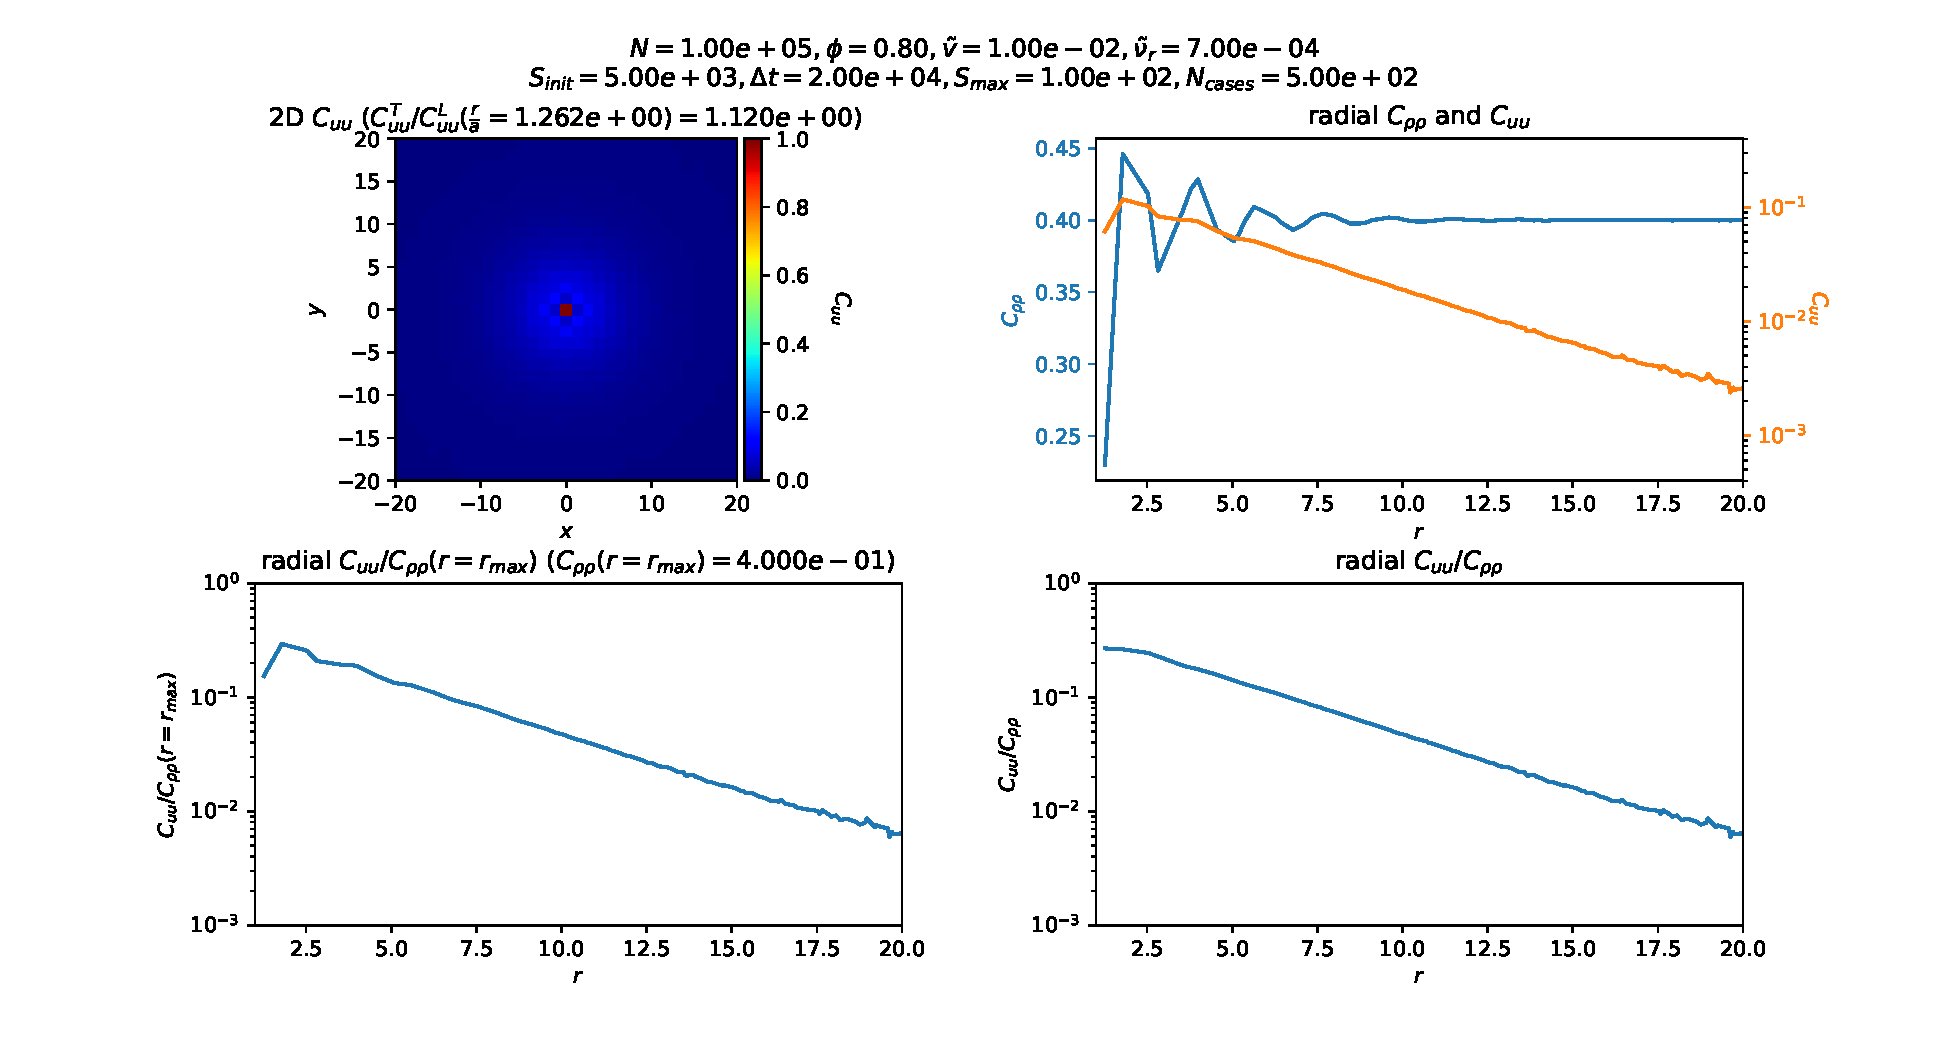
\includegraphics[width=\textwidth]{figures/figs/Cuub_Dk8000_Vj1000_Rh7000_Nq1000_Io5000_Tn2000_Mn1000_Cn5000_LINLOG.eps}
\caption{Comparison plots of displacement correlation $C_{uu}(r, \Delta t)$, density correlation $C_{\rho\rho}(r)$, and their ratio. \textbf{(top left)} 2D map of displacement correlation $C_{uu}(\vec{r} \equiv (x, y), \Delta t)$. We note the circular symmetry of this 2D map, which motivates our isotropy hypothesis. \textbf{(top right)} Displacement correlation $C_{uu}(r, \Delta t)$ and density correlation $C_{\rho\rho}(r)$. \textbf{(bottom left)} Displacement correlation $C_{uu}(r, \Delta t)$ divided by the plateau value of the density correlation, $C_{\rho\rho}(r = r_{max}) = 4\cdot10^{-1}$. \textbf{(bottom right)} Ratio of the displacement and density correlation.}
\label{cuu_oscillations}
\end{figure}

We note that while increasing $N_{cases}$ increases the number of radii at which $C_{uu}(r \in \mathcal{R}, \Delta t)$ is calculated, it can also increase the number of boxes with no particles, hence with $\vec{u} = \vec{0}$ according to equation \ref{u_to_grid}. At low radii $r \in \mathcal{R}$, $C_{uu}(r, \Delta t)$ will then be affected by the discrete nature of the system. Consequences of this are lower values of the computed correlation and unphysical oscillations, as illustrated by figure \ref{cuu_oscillations}.\\

To take this effect into account, we introduce $\forall m$, the density grid $(\rho_{kl}(t_m))_{1 \leq k, l \leq N_{cases}}$ associated to the displacement grid $(\vec{u}_{kl}(t_m, t_m + \Delta t))_{1 \leq k, l \leq N_{cases}}$ such that
\begin{equation}
\forall k, l,~ \rho_{kl}(t_m) = \begin{cases} 1 &\text{ if } \vec{u}_{kl}(t_m, t_m + \Delta t) \neq \vec{0} \\ 0 &\text{ if } \vec{u}_{kl}(t_m, t_m + \Delta t) = \vec{0} \end{cases}
\end{equation}
and compute the density correlation grid
\begin{equation}
C_{\rho\rho}(\vec{R}_{kl}) = \frac{\mathcal{F}^{-1}\left\{\left(\sum_m |\tilde{\rho}_{pq}(t_m)|^2\right)_{1 \leq p, q \leq N_{cases}}\right\}(\vec{R_{kl})}}{\sum_m\sum_{p, q} |\rho_{pq}(t_m)|^2}
\end{equation}
then its one-dimensional counterpart in the isotropy hypothesis
\begin{equation}
C_{\rho\rho}(r \in \mathcal{R}) = \left<C_{\rho\rho}(\vec{R}_{kl})\right>_{\vec{R}_{kl}, ||\vec{R}_{kl}||=r}
\end{equation}
which function is
\begin{itemize}
  \item constant and equal to 1 for low enough $N_{cases}$,
  \item and proportional to the pair-distribution function \cite{binder2011glassy21} for high enough $N_{cases}$.\\
\end{itemize}

We have verified that $C_{uu}(r, \Delta t)/C_{\rho\rho}(t)$ gave consistent results with any value of $N_{cases}$, thus indicating that this is the correct displacement correlation function within our computation method. Without further notice, we will then always consider this ratio rather than the bare displacement correlation function.\\

Our computation script is available at \href{https://github.com/yketa/active_particles/blob/master/analysis/cuu.py}{{\faGithub~ yketa/active\_particles/analysis/cuu.py}}.

\myparagraph{Displacement correlation comparison for a set of $(\phi, \tilde{v})$}

\begin{figure}[h!]
\centering
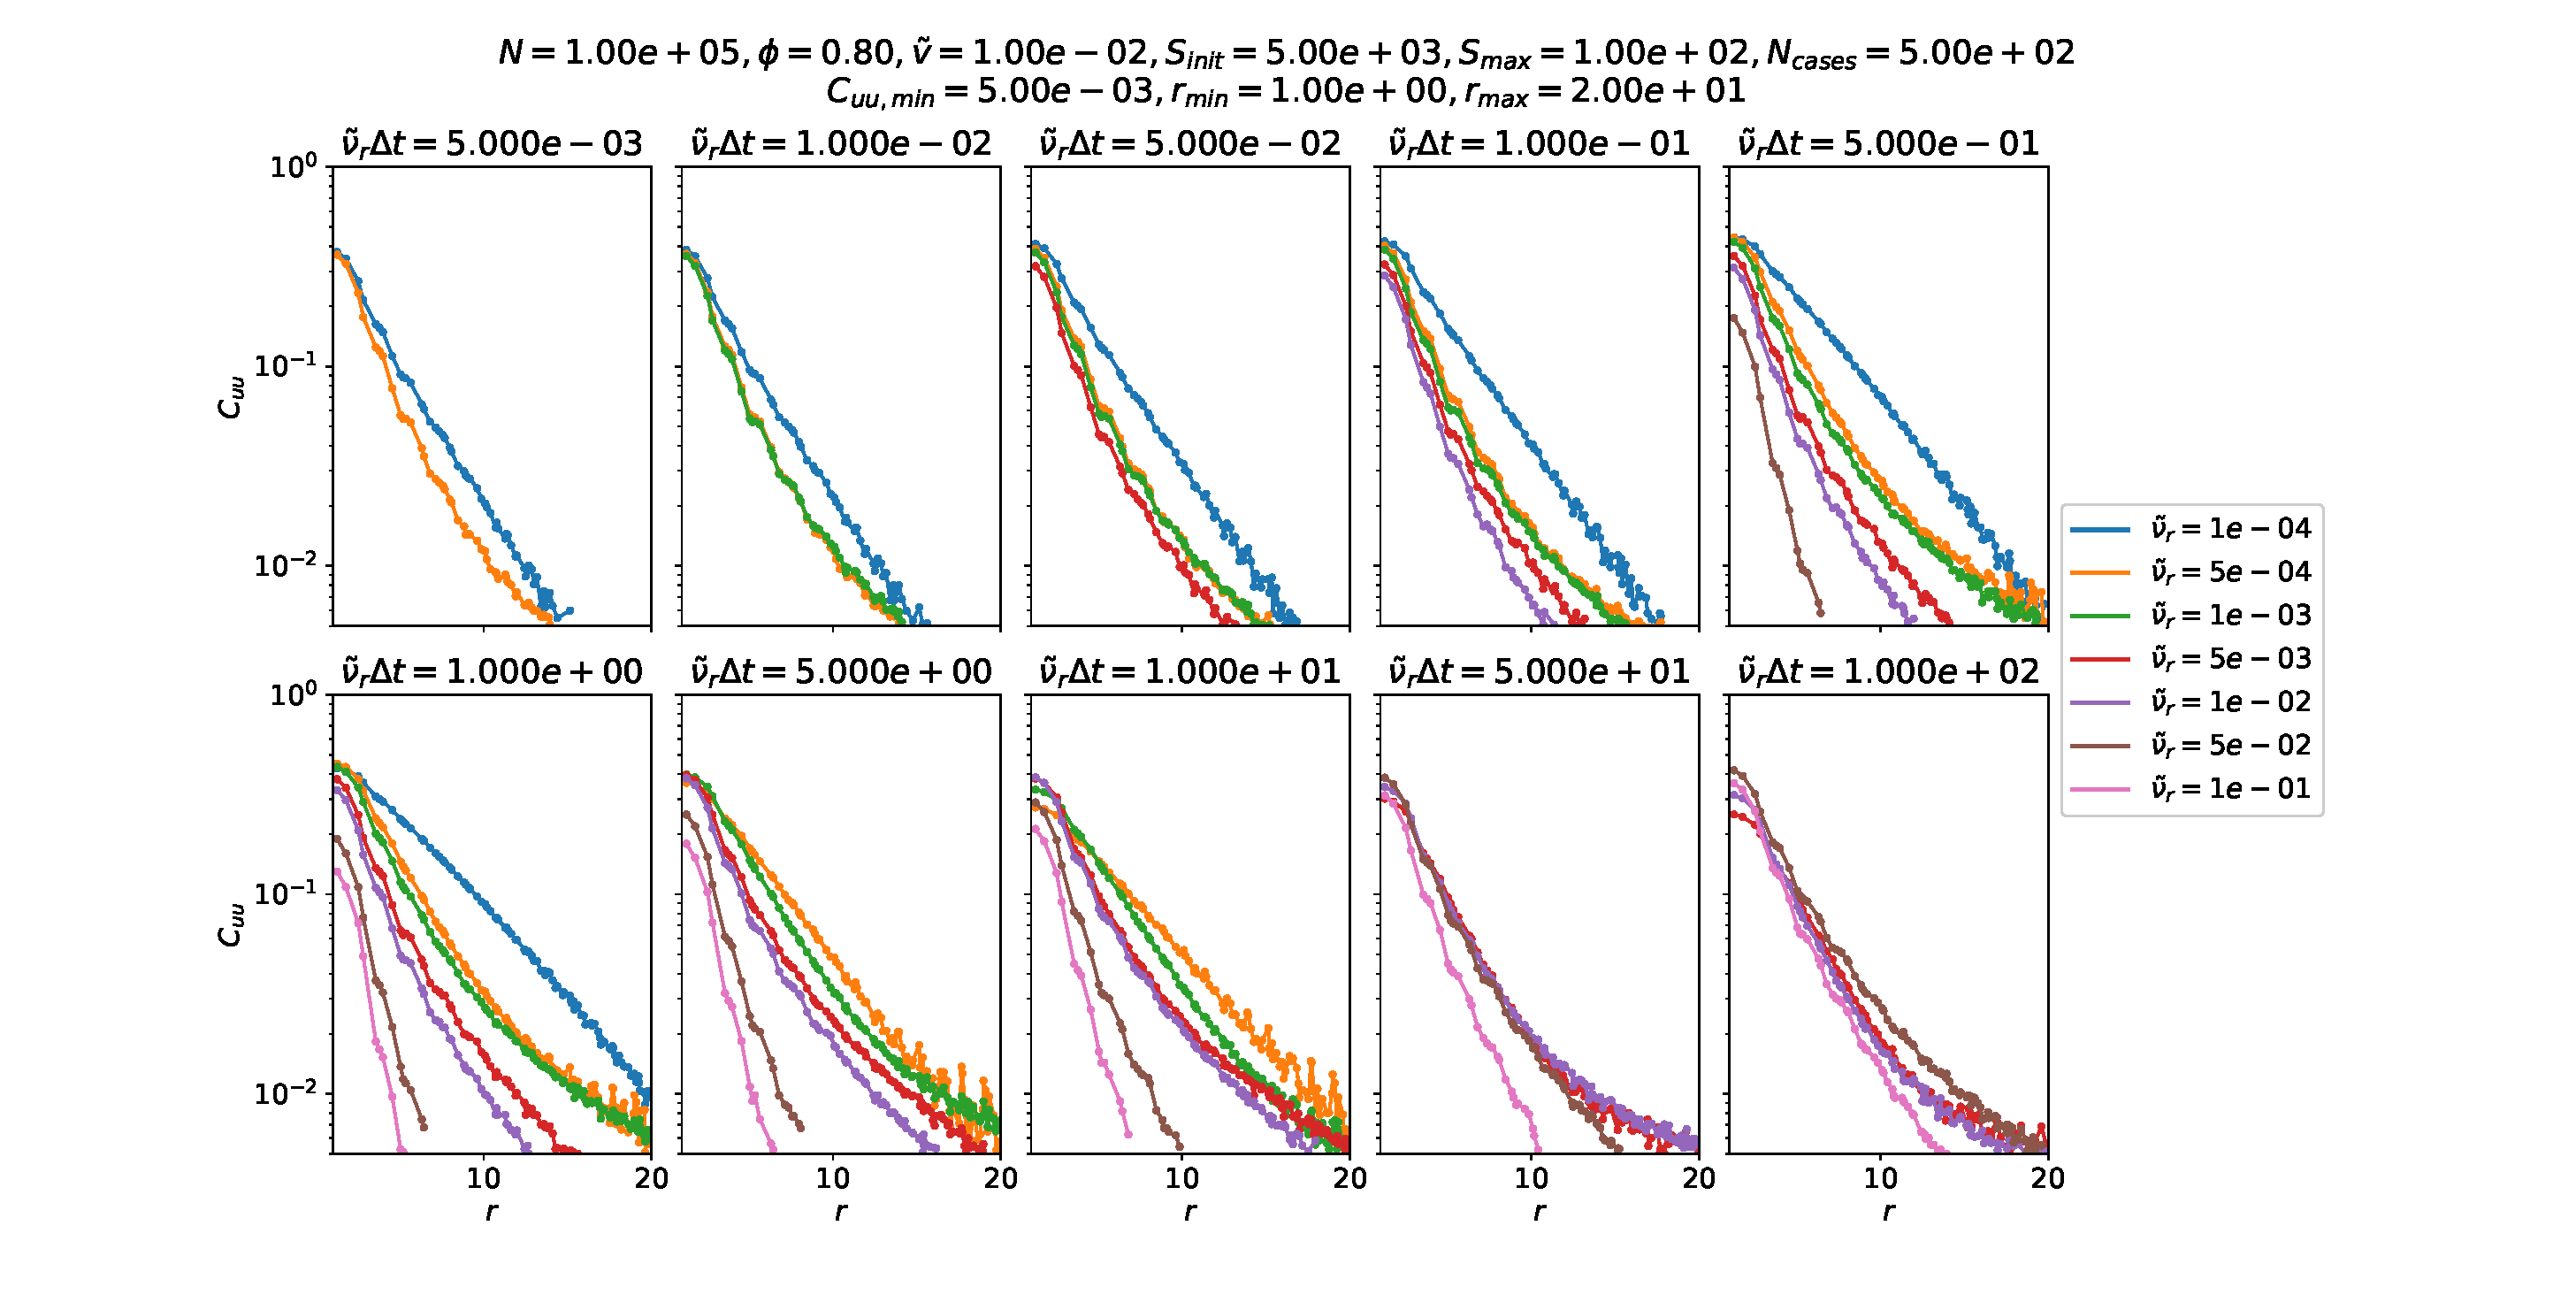
\includegraphics[width=\textwidth]{figures/figs/Cuu_comparison_Dk8000_Vj1000_Nq1000_Cn5000_LINLOG.eps}
\caption{Comparison plot of displacement correlation functions $C_{uu}(r, \Delta t)$ as defined by equation \ref{Cuu}, at packing fraction $\phi = 0.80$ and self-propulsion velocity $\tilde{v} = 1\cdot10^{-2}$, for different values of the rotational diffusion rate $\tilde{\nu}_r$. Each panel corresponds to an unique value of the product $\tilde{\nu}_r\Delta t$.}
\label{cuu_comparison}
\end{figure}

We observe in figure \ref{cuu_comparison} that for $\tilde{\nu}_r\Delta t < 1\cdot10^2$ we have $\forall r$ that the displacement correlation function at fixed $\tilde{\nu}_r \Delta t$, $C_{uu}(r, \tilde{\nu}_r \Delta t)$, is an increasing function of decreasing rotational diffusion rate $\tilde{\nu}_r$ (\textit{i.e.}, increasing persistence time $\tau_r$ and P\'eclet number $\text{Pe}$). We thus have for low enough $\tilde{\nu}_r\Delta t$ that the spatial extent of the displacement correlation function increases with activity, which is what we expected from the analysis of figure \ref{displacement_maps}.\\

However, we see for the highest value of $\tilde{\nu}_r\Delta t$ that this comparison becomes trickier. Curves actually cross, so what would be a correct definition of the "spatial extent" of the displacement correlation function which would be relevant in this case? Moreover, we stress that systematically comparing this amount of curves for each pair $(\phi, \tilde{v})$ and for all possible values of $\tilde{\nu}_r\Delta t$ is difficultly doable. We introduce in section \ref{section:cooperativity} the cooperativity which should solve both these issues.

\section{Cooperativity}
\label{section:cooperativity}

\subsection{Cooperativity}

Inspired by \cite{wysocki2014cooperative, doliwa2000cooperativity}, we introduce the cooperativity, $\chi$, linked to the displacement correlation, for a system within a square box of length $L$
\begin{equation}
\chi(\Delta t) = \frac{1}{L^2} \int_{r_{min}}^{r_{max}} dr~ 2\pi r~ C_{uu}(r, \Delta t)
\label{chi}
\end{equation}
with $r_{min}$ close to the average particle separation $a$ and $r_{max}$ such that $C_{uu}(r > r_{max}, \Delta t)$ is negligible.\\

This quantity is a global measure of cooperative motion and represents the average proportion of particles acting as coherently moving neighbours \cite{doliwa2000cooperativity}. It is thus a measure of the dynamic heterogeneity \cite{cavagna2009supercooled}.\\

At short times, particles move independently of each others in their own cage, which leads to low displacement correlations $C_{uu}(r, \Delta t)$ and thus low cooperativity $\chi(\Delta t)$. As times increases, they feel the motion of their neighbours and displacements become correlated over an increasing length scale which leads to an increasing cooperativity. At high times, we expect the motion of two initially neighbouring particles to become uncorrelated, thus decreasing the cooperativity. We then expect the curves of $\chi(\Delta t)$ to be bell-shaped \cite{wysocki2014cooperative, cavagna2009supercooled}. The positions of their maxima will tell us about the time scales over which the motion of the particles is correlated, and their amplitudes about the number of particles involved in cooperative motion.

\subsection{Varying roational diffusion rate $\tilde{\nu}_r$}

\begin{figure}[h!]
\centering
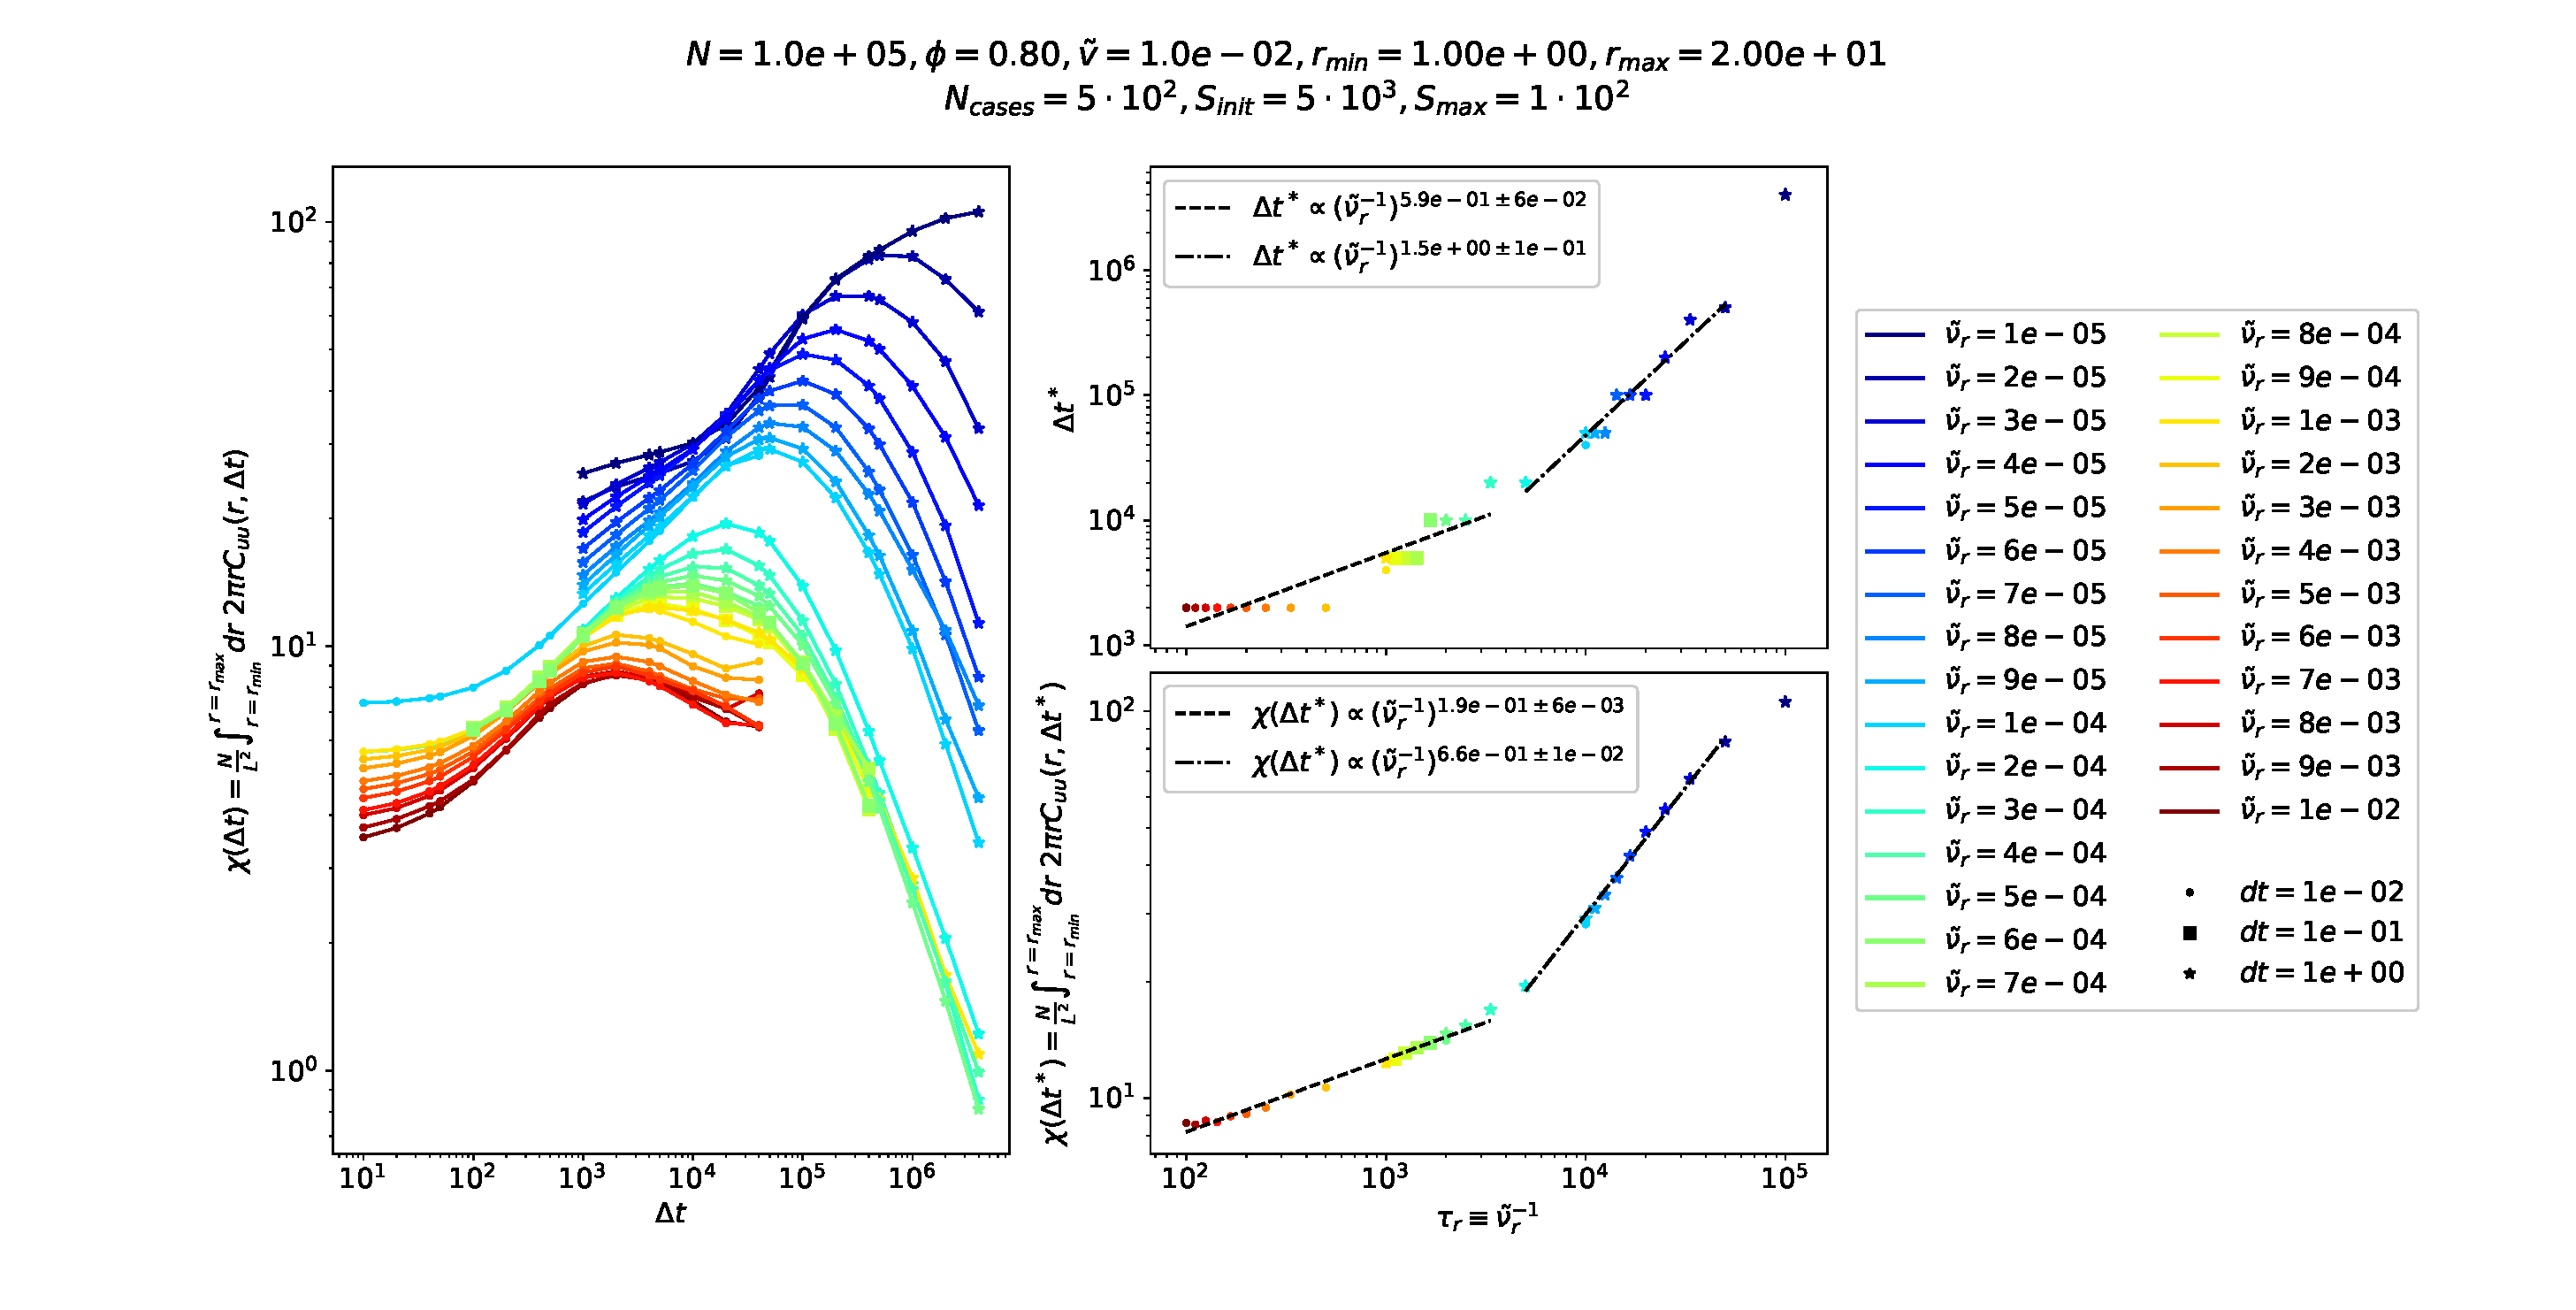
\includegraphics[width=\textwidth]{figures/figs/intCuu_dt_Dk8000_Vj1000_Nq1000_Io5000_Mn1000_Cn5000_RMINl1000_RMAXm2000.eps}
\caption{Cooperativities $\chi(\Delta t)$ as defined by equation \ref{chi}, at packing fraction $\phi = 0.80$ and self-propulsion velocity $\tilde{v} = 1\cdot10^{—2}$, for different values of the rotational diffusion rate $\tilde{\nu}_r$. Quantity $dt$ refers to the time step used in the simulation. \textbf{(left)} Cooperativity as a function of lag time $\chi(\Delta t)$. Each continuous line corresponds to a single simulation. \textbf{(top right)} Position $\Delta t^*$ of maximum cooperativity $\chi(\Delta t^*)$ as a function of the P\'eclet number $\text{Pe} = \tilde{v}/\tilde{\nu}_r$. Dashed lines correspond to arbitrary power law fits. \textbf{(bottom right)} Amplitude $\chi(\Delta t^*)$ of maximum cooperativity as a function of the P\'eclet number $\text{Pe} = \tilde{v}/\tilde{\nu}_r$. Dashed lines correspond to arbitrary power law fits.}
\label{chi_dr_dt}
\end{figure}

We have in figure \ref{chi_dr_dt} that $\chi(\Delta t)$ curves are indeed bell-shaped as we predicted.\\

For any lag time $\Delta t$, we have that the number of coherently moving neighbours is an increasing function of increasing activity (\textit{i.e.}, increasing persistence time $\tau_r$ and P\'eclet number $\text{Pe}$, and decreasing rotational diffusion rate $\tilde{\nu}_r$). Moreover, we have
\begin{itemize}
  \item that the maximum number of coherently moving neighbours, $\chi(\Delta t^*)$, is a strictly increasing function of the activity, indicating that dynamic heterogeneity grows as the activity grows,
  \item and that the lag time at which this maximum cooperative motion occurs, $\Delta t^*$, is also a strictly increasing function of the activity, which is consistent with the physical intuition that a cooperative behaviour involving a greater number of particles must happen over a greater time scale.\\
\end{itemize}

We also note that there is a clear transition at $\text{Pe}_t \approx 10^{1.5}$ between two regimes wherein the increases of both $\Delta t^*$ and $\chi(\Delta t^*)$ are algebraic in $\text{Pe}$ and with different slopes. This transition value of the P\'eclet number is consistent with the approximate transition value between the fluid states and the phase separated states inferred from the local packing fraction histogram in figure \ref{philoc_dr}.\\

\begin{figure}[h!]
\centering
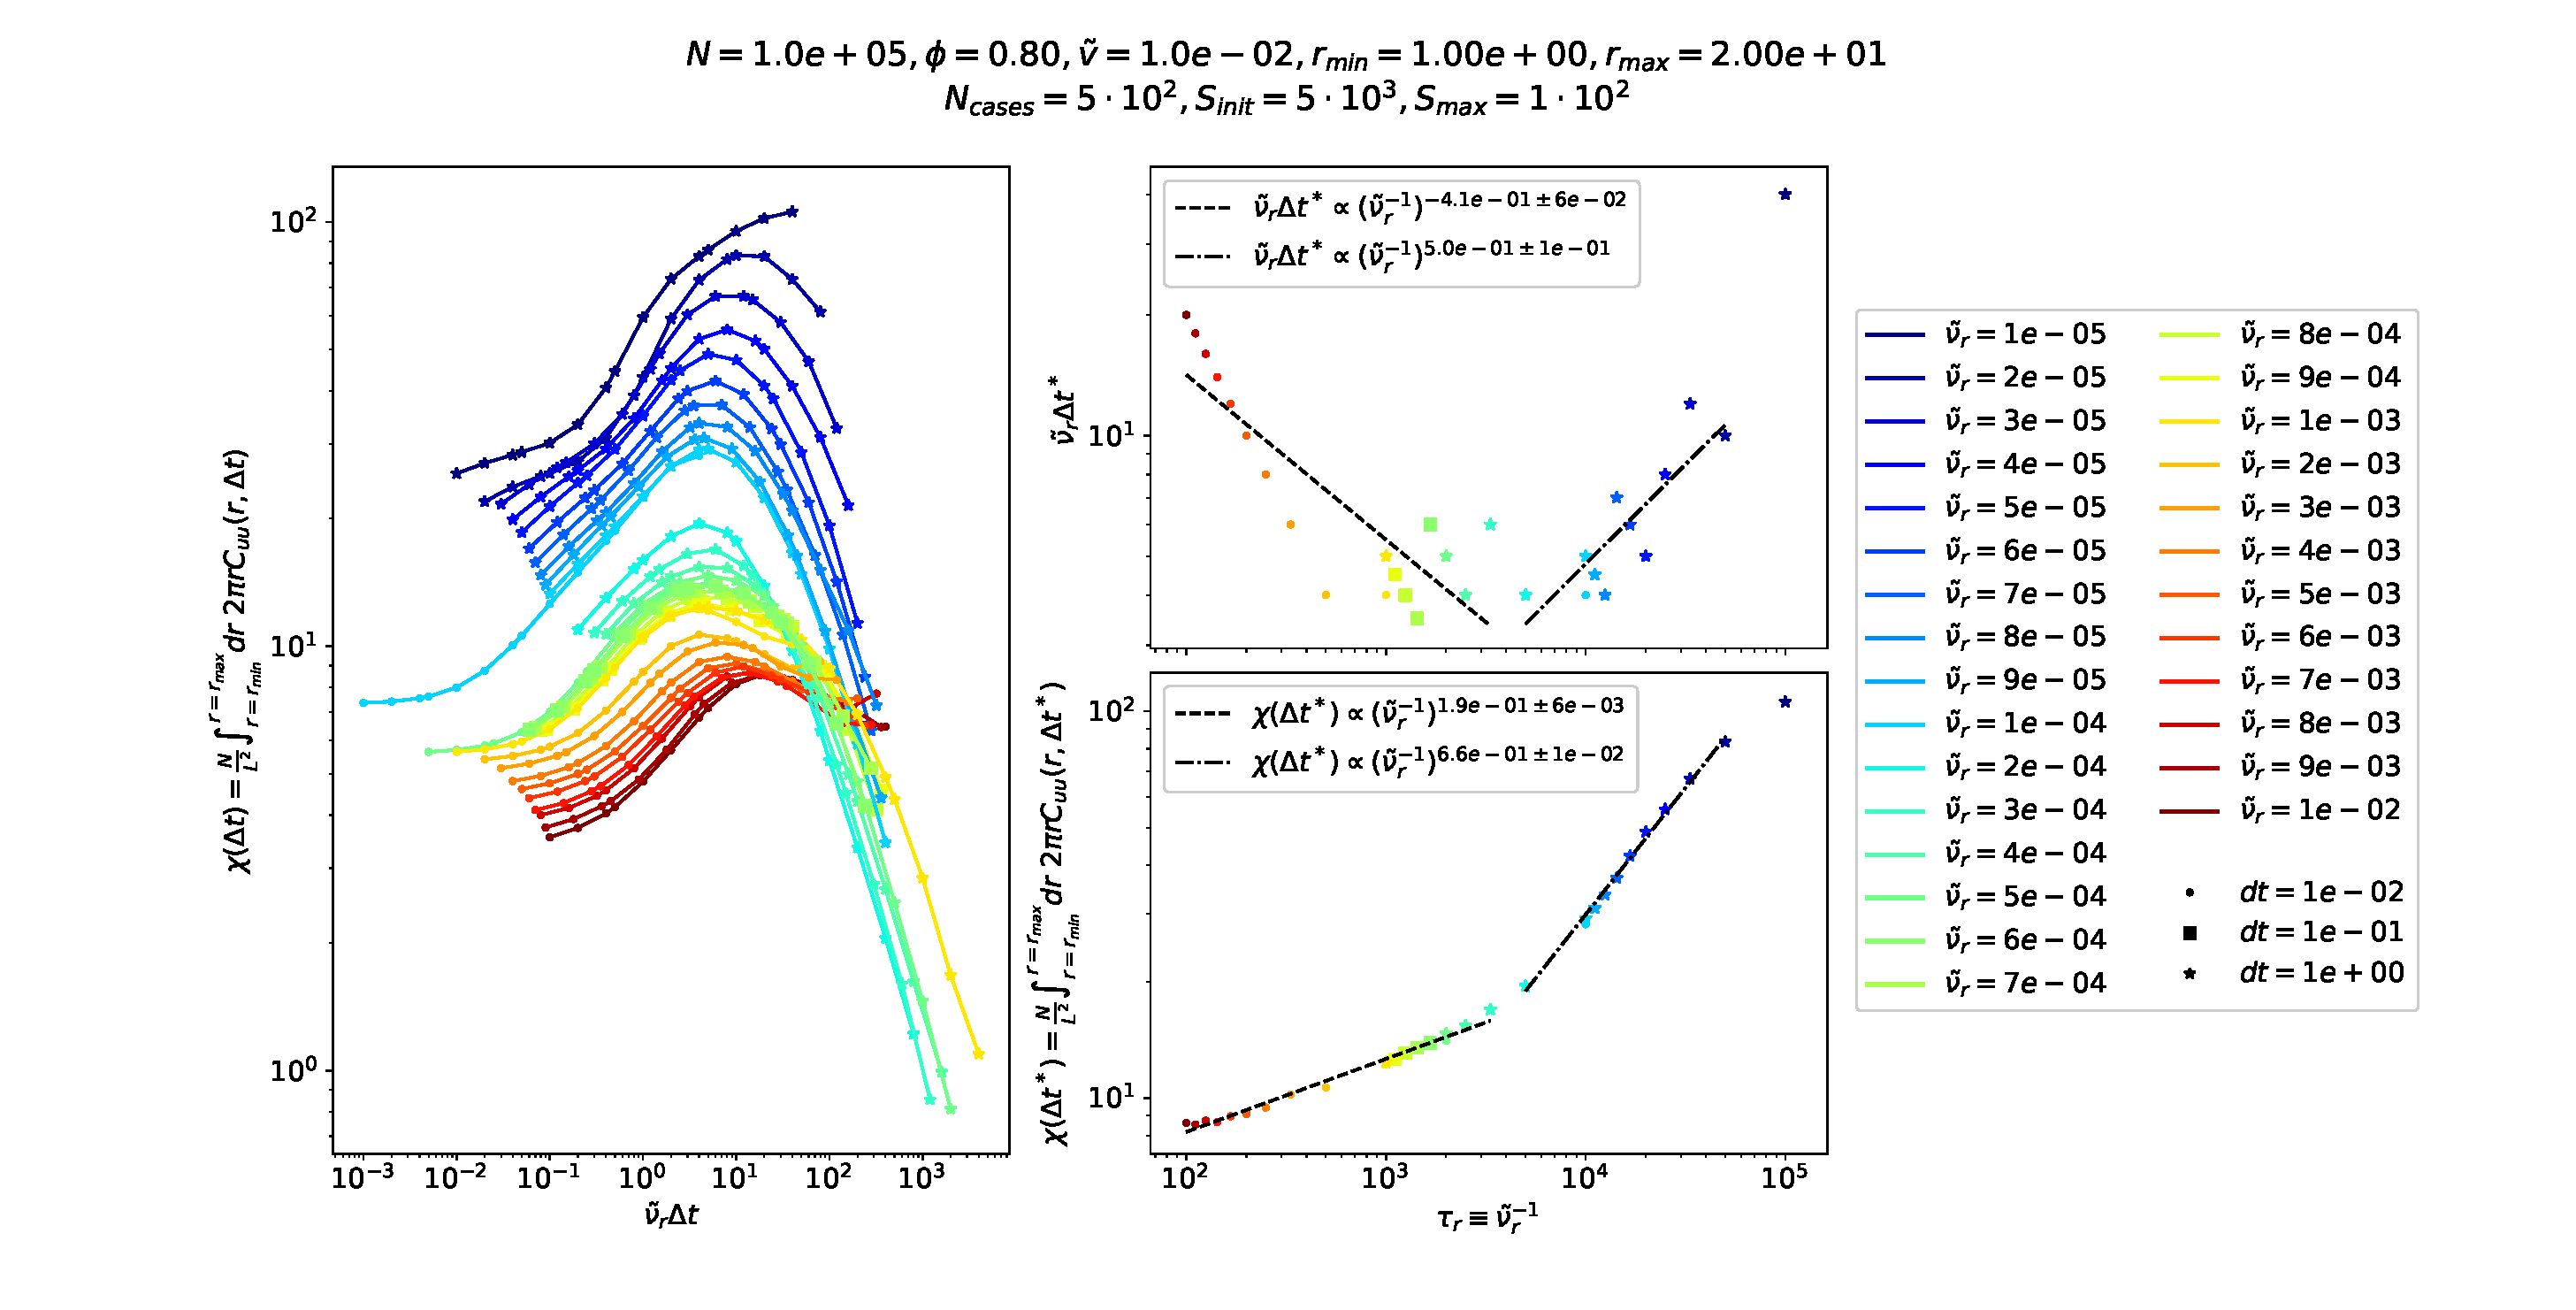
\includegraphics[width=\textwidth]{figures/figs/intCuu_Dk8000_Vj1000_Nq1000_Io5000_Mn1000_Cn5000_RMINl1000_RMAXm2000.eps}
\caption{Cooperativities $\chi(\Delta t)$ as defined by equation \ref{chi}, at packing fraction $\phi = 0.80$ and self-propulsion velocity $\tilde{v} = 1\cdot10^{—2}$, for different values of the rotational diffusion rate $\tilde{\nu}_r$. Quantity $dt$ refers to the time step used in the simulation. \textbf{(left)} Cooperativity as a function of the product of lag time and rotational diffusion rate $\chi(\tilde{\nu}_r \Delta t)$. Each continuous line corresponds to a single simulation. \textbf{(top right)} Position $\tilde{\nu}_r \Delta t^*$ of maximum cooperativity $\chi(\tilde{\nu}_r \Delta t^*)$ as a function of the P\'eclet number $\text{Pe} = \tilde{v}/\tilde{\nu}_r$. Dashed lines correspond to arbitrary power law fits. \textbf{(bottom right)} Amplitude $\chi(\Delta t^*)$ of maximum cooperativity as a function of the P\'eclet number $\text{Pe} = \tilde{v}/\tilde{\nu}_r$. Dashed lines correspond to arbitrary power law fits.}
\label{chi_dr}
\end{figure}

We observe in figure \ref{chi_dr} that for $\tilde{\nu}_r \Delta t \lessapprox 10^2$, $\chi(\tilde{\nu}_r \Delta t)$, \textit{i.e.} the number of coherently moving neighbours, is an increasing function of the activity, which is consistent with what we had observed in figure \ref{displacement_maps}.\\

We have seen in section \ref{subsection:self_propulsion_mechanism} that the persistence time $\tau_r$ qualitatively represents the amount of time during which the self-propulsion velocity of particles remains oriented in the same direction. Thus, $\tilde{\nu}_r \Delta t = \Delta t/\tau_r$ represents the number of reorientations of this self-propulsion velocity. We have in figure \ref{chi_dr} that this number of reorientations corresponding to the time scale of maximum cooperativity, $\tilde{\nu}_r \Delta t^*$, is roughly a decreasing function of the P\'eclet number $\text{Pe}$ for $\text{Pe} \lessapprox \text{Pe}_t$ and an increasing function of $\text{Pe}$ for $\text{Pe} \gtrapprox \text{Pe}_t$, and is therefore minimum at the transition value $\text{Pe}_t$. The origin of this behaviour is still an open question for us.\\

The quickly increasing dynamic heterogeneity, as measured by the maximum cooperativity $\chi(\Delta t^*)$, with increasing activity in the phase separated regime is reminiscent of the behaviour of a glass-forming material when decreasing its temperature \cite{berthier2011dynamic, cavagna2009supercooled}. We can then look for other evidence of such behaviour, \textit{e.g.} by looking at the mean square displacement as we have done in section \ref{subsection:phase_diagram} (figure \ref{msd_phi}).\\

\begin{figure}[h!]
\centering
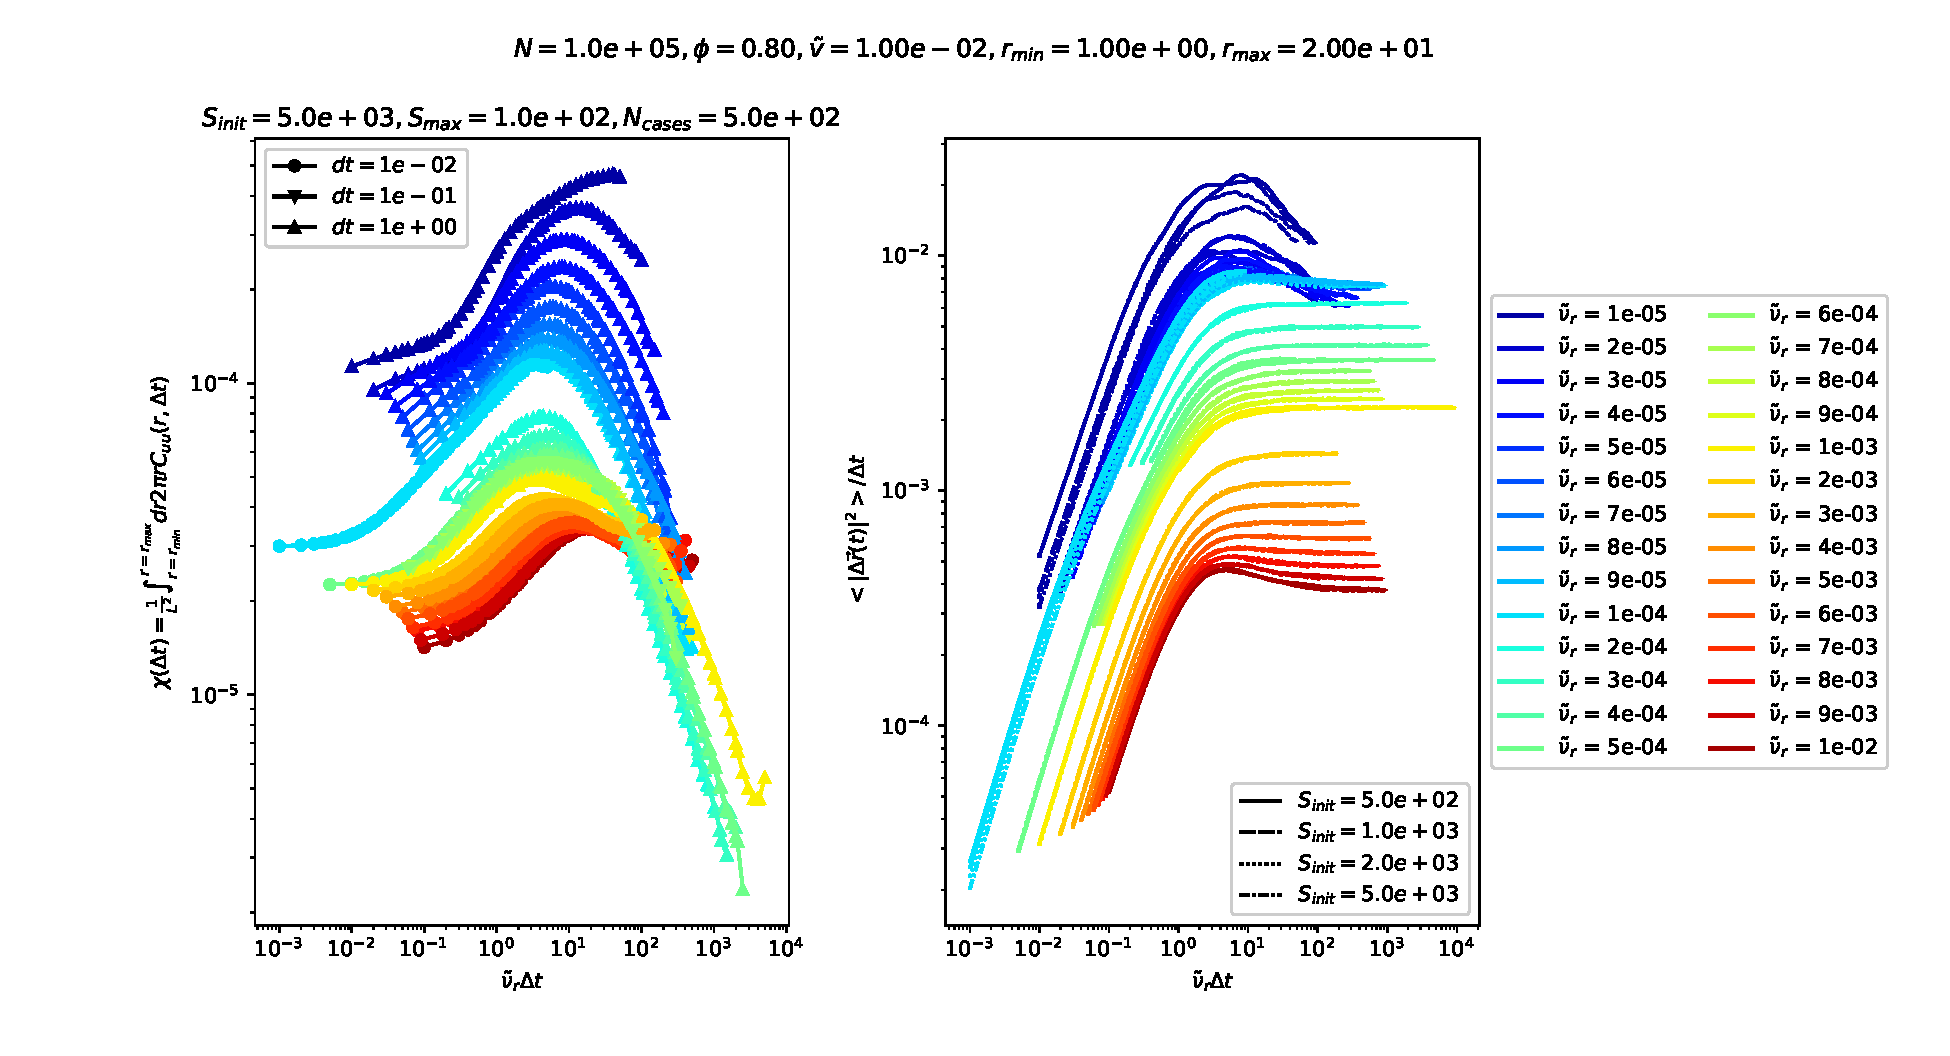
\includegraphics[width=\textwidth]{figures/figs/intCuu_msdt_Dk8000_Vj1000_Nq1000_Io5000_Mn1000_Cn5000_RMINl1000_RMAXm2000.eps}
\caption{Cooperativities $\chi(\Delta t)$ as defined by equation \ref{chi}, and mean square displacements as defined by equation \ref{msd_ensemble}, at packing fraction $\phi = 0.80$ and self-propulsion velocity $\tilde{v} = 1\cdot10^{—2}$, for different values of the rotational diffusion rate $\tilde{\nu}_r$. Quantity $dt$ refers to the time step used in the simulation. \textbf{(left)} Cooperativity as a function of the product of lag time and rotational diffusion rate $\chi(\tilde{\nu}_r \Delta t)$. Each continuous line corresponds to a single simulation. \textbf{(right)} Ratio of mean square displacement $\left<|\Delta\vec{r}(\Delta t)|^2\right>$ and lag time $\Delta t$ as a function of lag time $\Delta t$. $S_{init}$ refers to the frame of the simulation considered as the time $t=0$ to compute mean square displacements.}
\label{chi_dr_msd}
\end{figure}

We have in figure \ref{chi_dr_msd} that, for $\text{Pe} \lessapprox \text{Pe}_t$, $\lim_{t \rightarrow +\infty} \left<|\Delta\vec{r}(t)|^2\right> = \text{cst}$, indicating a diffusive behaviour at high times which is what we would expect for fluid states \cite{binder2011glassy}. For $\text{Pe} \gtrapprox \text{Pe}_t$, there is a clear -- and possibly transient -- subdiffusive behaviour, such as observed in glasses, as we discussed in section \ref{subsection:phase_diagram}.\\

An other evidence of glassiness is ageing \cite{courtland2002direct}, as illustrated by the dependence of mean square displacement curves $\left<|\Delta\vec{r}(t)|^2\right>$ with the simulation frame considered as initial in their calculation $S_{init}$.

\subsection{Varying self-propulsion velocity $\tilde{v}$}

\begin{figure}[h!]
\centering
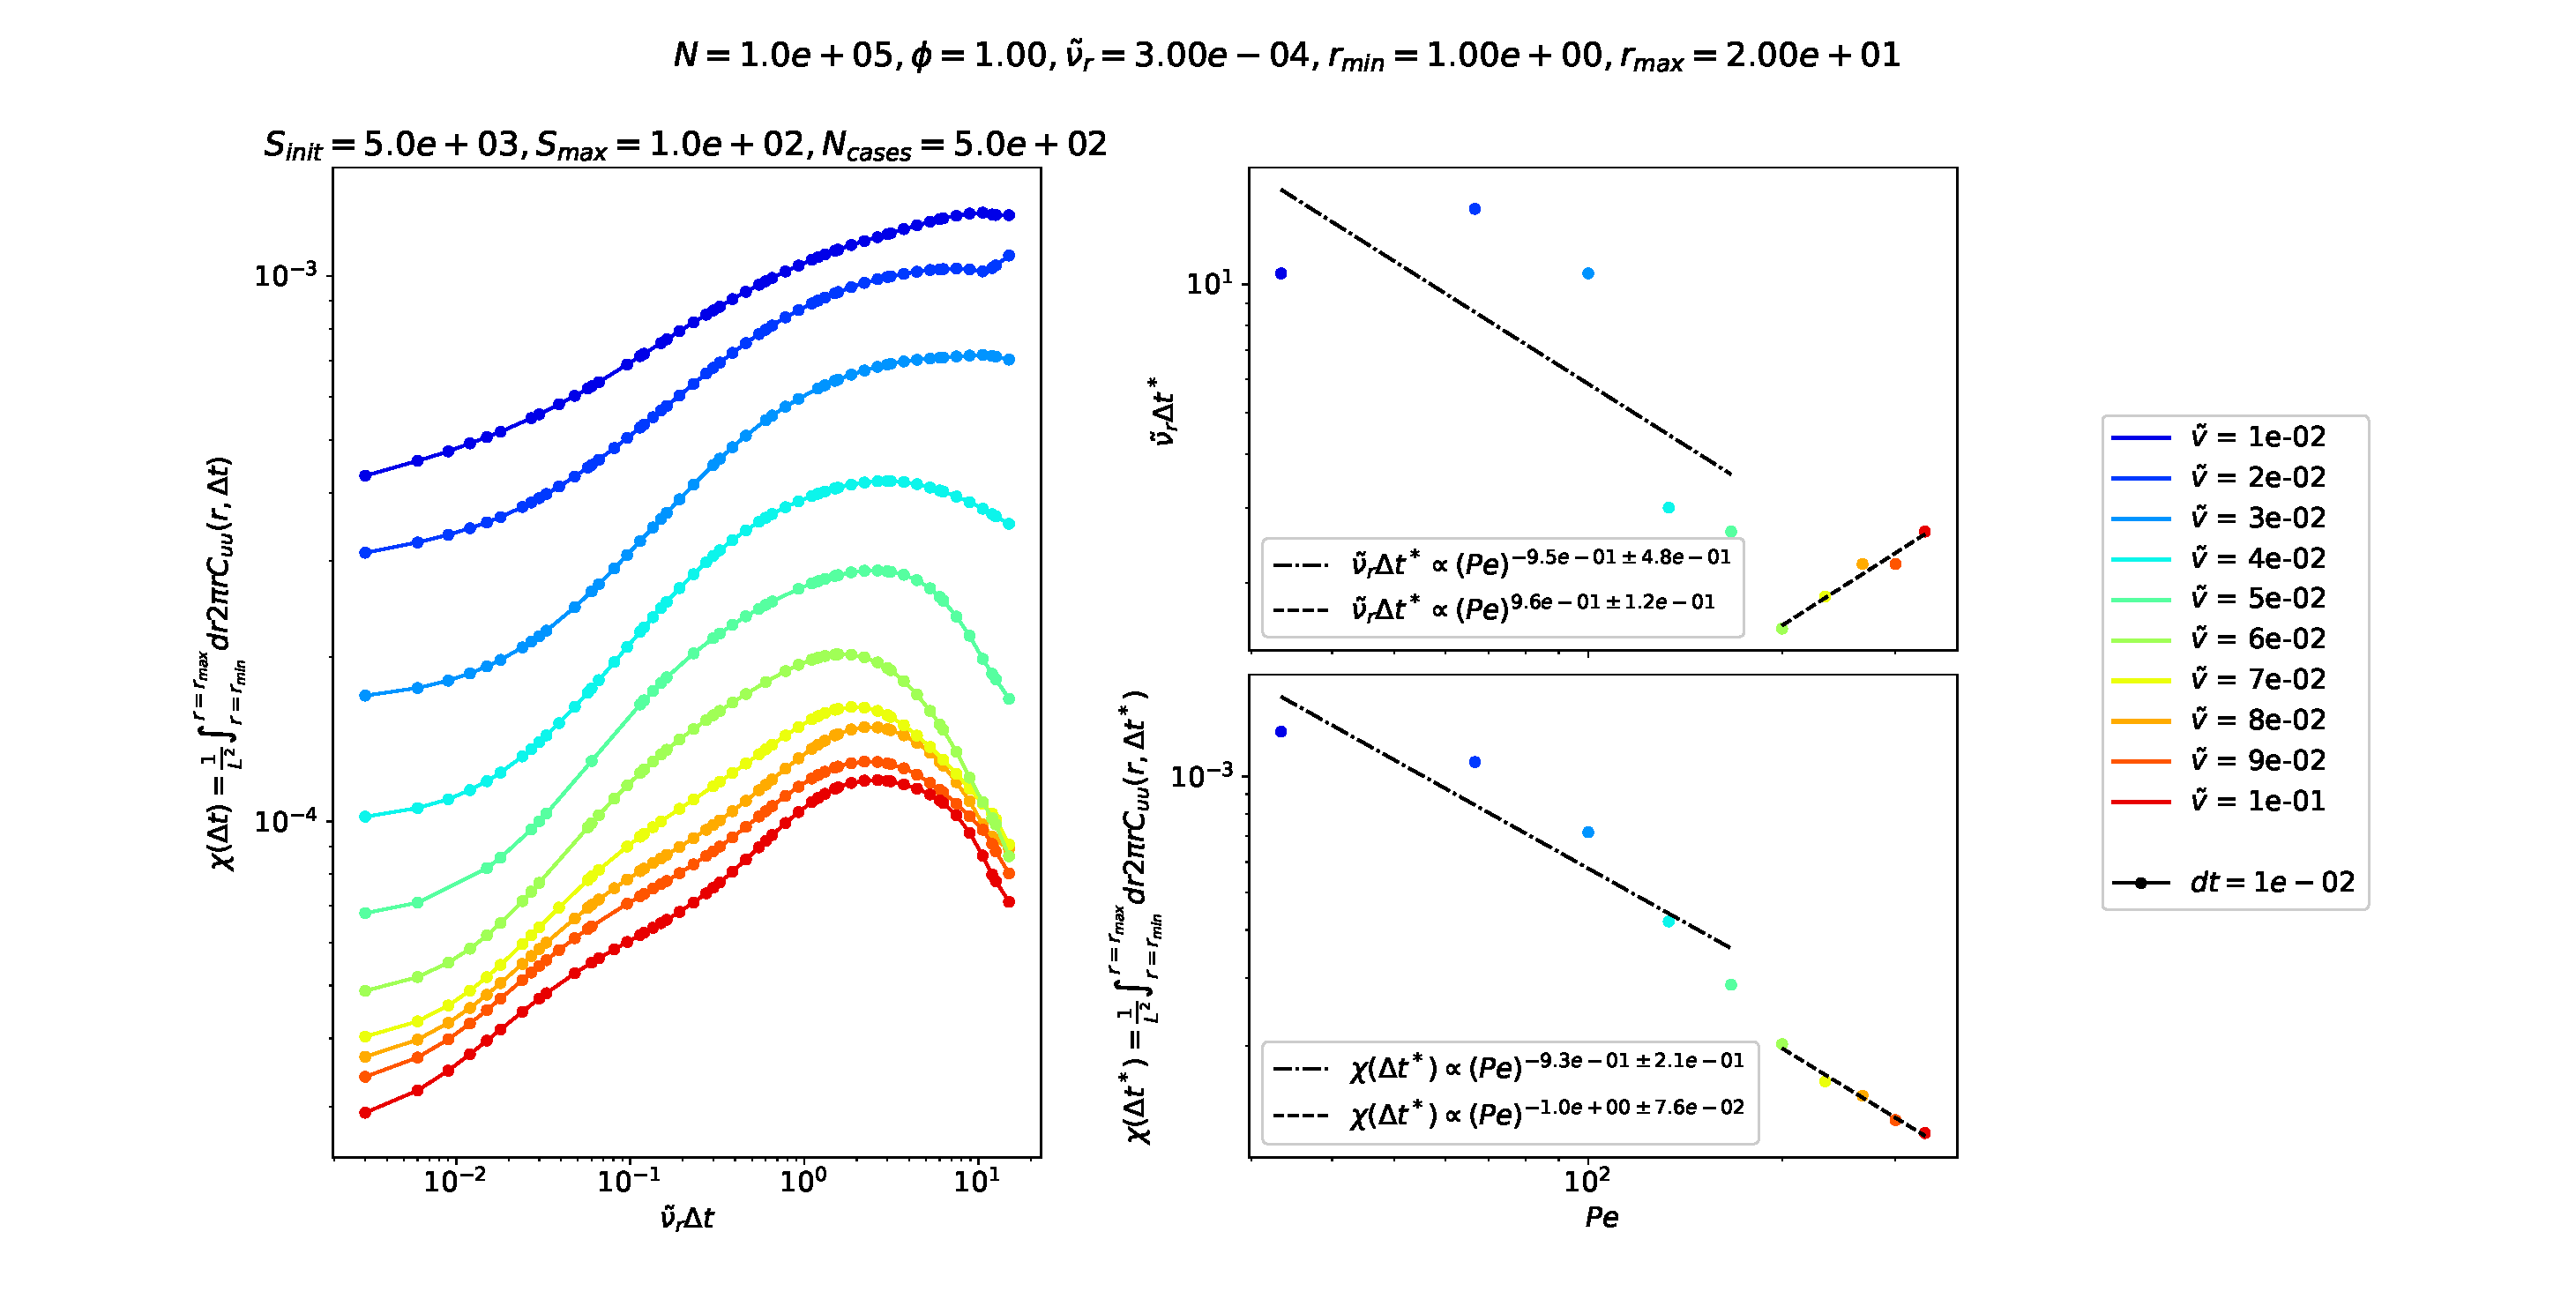
\includegraphics[width=\textwidth]{figures/figs/intCuu_Dk8000_Rh3000_Nq1000_Io5000_Mn1000_Cn5000_RMINl1000_RMAXm2000.eps}
\caption{Cooperativities $\chi(\Delta t)$ as defined by equation \ref{chi}, at packing fraction $\phi = 1.00$ and rotational diffusion rate $\tilde{\nu}_r = 3\cdot10^{—4}$, for different values of the self-propulsion velocity $\tilde{v}$. Quantity $dt$ refers to the time step used in the simulation. \textbf{(left)} Cooperativity as a function of the product of lag time and rotational diffusion rate $\chi(\tilde{\nu}_r \Delta t)$. Each continuous line corresponds to a single simulation. \textbf{(top right)} Position $\tilde{\nu}_r \Delta t^*$ of maximum cooperativity $\chi(\tilde{\nu}_r \Delta t^*)$ as a function of the P\'eclet number $\text{Pe} = \tilde{v}/\tilde{\nu}_r$. Dashed lines correspond to arbitrary power law fits. \textbf{(bottom right)} Amplitude $\chi(\Delta t^*)$ of maximum cooperativity as a function of the P\'eclet number $\text{Pe} = \tilde{v}/\tilde{\nu}_r$. Dashed lines correspond to arbitrary power law fits.}
\label{chi_v}
\end{figure}

\begin{figure}[h!]
\centering
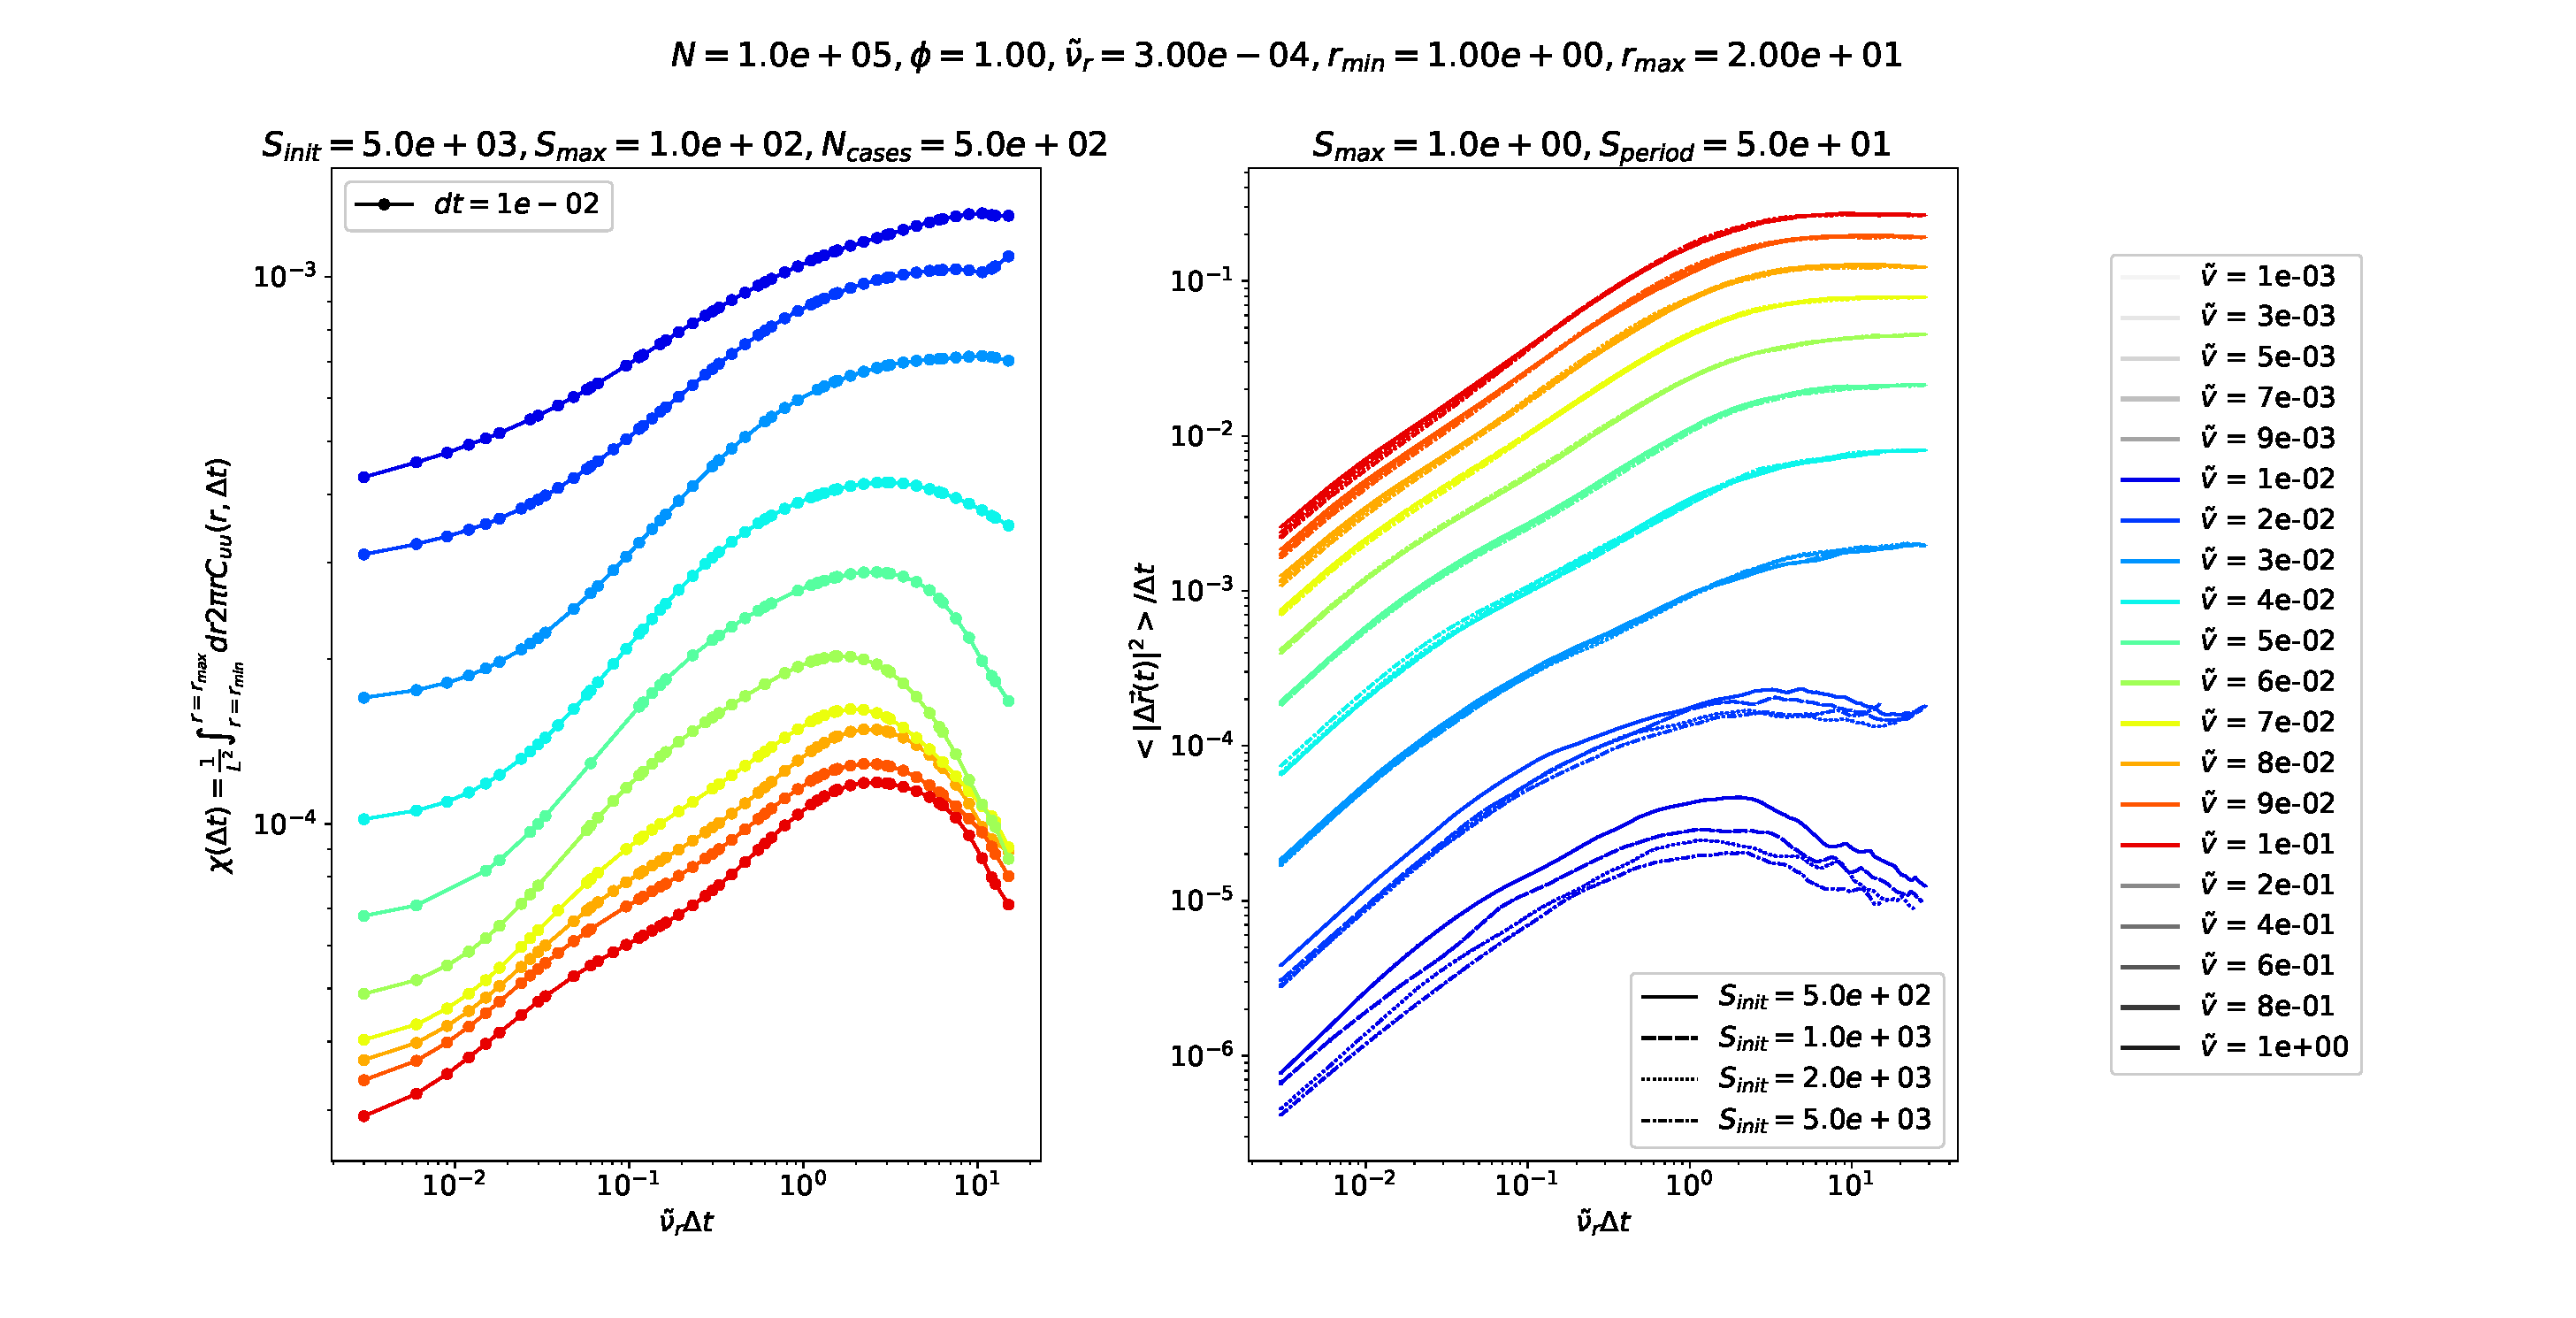
\includegraphics[width=\textwidth]{figures/figs/intCuu_msdt_Dk8000_Rh3000_Nq1000_Io5000_Mn1000_Cn5000_RMINl1000_RMAXm2000.eps}
\caption{Cooperativities $\chi(\Delta t)$ as defined by equation \ref{chi}, and mean square displacements as defined by equation \ref{msd_ensemble}, at packing fraction $\phi = 1.00$ and rotational diffusion rate $\tilde{\nu}_r = 3\cdot10^{—4}$, for different values of the self-propulsion velocity $\tilde{v}$. Quantity $dt$ refers to the time step used in the simulation. \textbf{(left)} Cooperativity as a function of the product of lag time and rotational diffusion rate $\chi(\tilde{\nu}_r \Delta t)$. Each continuous line corresponds to a single simulation. \textbf{(right)} Ratio of mean square displacement $\left<|\Delta\vec{r}(\Delta t)|^2\right>$ and lag time $\Delta t$ as a function of lag time $\Delta t$. $S_{init}$ refers to the frame of the simulation considered as the time $t=0$ to compute mean square displacements.}
\label{chi_v_msd}
\end{figure}

Figure \ref{chi_v} presents the few results we have so far for the cooperativity at fixed $(\phi, \tilde{\nu}_r)$ and varying self-propulsion velocity $\tilde{v}$. Despite the great dispersion of the values of the number of reorientations corresponding to the time scale of maximum cooperativity $\tilde{\nu}_r \Delta t^*$ around our power law fits, we hypothesise that there is a transition at $\text{Pe}_t \approx 2\cdot10^2$ between regimes of decreasing and increasing $\tilde{\nu}_r \Delta t^*$ with increasing $\text{Pe}$, respectively for $\text{Pe} \lessapprox \text{Pe}_t$ and $\text{Pe} \gtrapprox \text{Pe}_t$. We first note that this transition value $\text{Pe}$ of the P\'eclet number is consistent with the approximate transition value between the fluid states and the phase separated states inferred from the local packing fraction histogram in figure \ref{philoc_v}. We then highlight that this non-monotonous behaviour of $\tilde{\nu}_r \Delta t^*(\text{Pe})$ is similar to what has been observed when transitioning from the fluid regime to the phase separated regime by varying the rotational diffusion rate $\tilde{\nu}_r$ (see figure \ref{chi_dr}).\\

We also see in figure \ref{chi_v} that the maximum number of coherently moving neighbours, $\chi(\Delta t^*)$ is a strictly decreasing function of increasing P\'eclet number $\text{Pe}$. This is not only the exact opposite behaviour that what was observed when varying the rotational diffusion rate $\tilde{\nu}_r$ (see figure \ref{chi_dr}), this is also quite counter intuitive. Indeed, we remind that the P\'eclet number represents the dimensionless distance travelled by a single particle before its self-propulsion orientation decorrelates. We would then expect that the greater this number is, the larger the cluster of coherently moving neighbours get. The origin of this behaviour is still an open question for us.\\

What is however clear from these findings is that the sole P\'eclet number $\text{Pe}$ is not enough to characterise our model system, contrarily to what has been considered in \cite{wysocki2014cooperative}.\\

We observe in figure \ref{chi_v_msd} both subdiffusive and ageing behaviours in mean square displacements for $\tilde{v} = 1\cdot10^{-2}, 2\cdot10^{—2}$. This is consistent with the positions of these points in the phase diagram of figure \ref{phase_diagram} where they sit in the "frozen" states.\\

However, we see for the highest values of the self-propulsion velocity $\tilde{v}$ (\textit{i.e.}, for the highest values of the P\'eclet number $\text{Pe}$) that the mean square displacements show no sign of either subdiffusive or ageing behaviours, even though we had observed it for $\text{Pe} \gtrapprox \text{Pe}_t$ when varying the rotational diffusion rate $\tilde{\nu}_r$ (see figure \ref{chi_dr_msd}).\\

Maybe the reason to this is that we are not deep enough in the phase separated regime. We hypothesise that, for higher values of the self-propulsion velocity $\tilde{v}$, the dynamic heterogeneity as measured by the maximum number of coherently moving neighbours $\chi(\Delta t^*)$ would eventually increase.

\section{Directional displacement correlation}
\label{section:directional_displacement_correlation}

\subsection{Directional displacement correlation}

\myparagraph{Definition}

We have seen the influence of activity on the cooperativity of the motion of particles as measured by the spatial extent of displacement correlation functions (section \ref{section:cooperativity}). We can now wonder if activity affects the correlations in the directions of motion of pairs of particles.\\

To this effect, we introduce the longitudinal and transversal displacement correlations \cite{weeks2007short, vasisht2018rate}
\begin{equation}
\begin{aligned}
C_{uu}^L(\Delta\vec{r}, \Delta t) &= \left<u_L(\vec{r} + \Delta \vec{r}, t, t + \Delta t)u_L(\vec{r}, t, t + \Delta t)\right>_{\vec{r}, t}\\
C_{uu}^T(\Delta\vec{r}, \Delta t) &= \left<\vec{u}_T(\vec{r} + \Delta \vec{r}, t, t + \Delta t)\cdot\vec{u}_T(\vec{r}, t, t + \Delta t)\right>_{\vec{r}, t}
\end{aligned}
\label{cuul_cuut}
\end{equation}
with $u_L(\vec{r}, t, t + \Delta t)$ the longitudinal displacement and $\vec{u}_T(\vec{r}, t, t + \Delta t)$ the transversal displacement, defined as
\begin{equation}
\vec{u}(\vec{r}, t, t + \Delta t) = \underbrace{\frac{\vec{u}(\vec{r}, t, t + \Delta t)\cdot\Delta\vec{r}}{||\Delta\vec{r}||}}_{\displaystyle u_L(\vec{r}, t, t + \Delta t)}\frac{\Delta\vec{r}}{||\Delta\vec{r}||} + \underbrace{\vphantom{\frac{\vec{u}(\vec{r}, t, t + \Delta t)\cdot\Delta\vec{r}}{||\Delta\vec{r}||}}\vec{u}(\vec{r}, t, t + \Delta t) - u_L(\vec{r}, t, t + \Delta t)\Delta\vec{r}}_{\displaystyle\vec{u}_T(\vec{r}, t, t + \Delta t)\perp\Delta\vec{r}}
\end{equation}
where $\vec{u}(\vec{r}, t, t + \Delta t)$ is the displacement vector of the particle at position $\vec{r}$ at time $t$ between times $t$ and $t + \Delta t$.\\

We are interested in the correlations in the directions of motion of pairs of \textit{neighbouring} particles, we will then only consider the values of the transversal and longitudinal displacement correlations at a fixed radius close to the interparticle distance $r \approx a$ in equation \ref{cuul_cuut}. Without further notice, we will use functions $C_{uu}^L(\Delta t)$ and $C_{uu}^T(\Delta t)$ of the sole lag time $\Delta t$.

\myparagraph{Computation details}

Longitudinal and transversal displacement correlations are calculated with the same routine as displacement correlations (see section \ref{displacement_correlation}). Our computation script is available at \href{https://github.com/yketa/active_particles/blob/master/analysis/cuu.py}{{\faGithub~ yketa/active\_particles/analysis/cuu.py}}.

\myparagraph{Raw data with varying rotational diffusion rate $\tilde{\nu}_r$}

We have that data in figure \ref{cuul_cuut_separate} is difficultly exploitable. $C_{uu}^L(\tilde{\nu}_r\Delta t)$ and $C_{uu}^T(\tilde{\nu}_r\Delta t)$ are non-monotonous and is hard to establish whether any of these approach a limiting curve in either low or high rotational diffusion rate $\tilde{\nu}_r$ limit.\\

Values of $C_{uu}^L(\Delta t^*)$ and $C_{uu}^T(\Delta t^*)$ for $\text{Pe} \lessapprox 10^1$ look well behaved and are an increasing function of the P\'eclet number for the former and more or less constant for the latter. However, for $\text{Pe} > 10^1$, it becomes trickier to make any assertion about the behaviour of these quantities.\\

We then propose to look not at the raw values of the longitudinal and transversal displacement correlations but at their ratio, as was done in \cite{vasisht2018rate}.

\begin{figure}[h!]
\centering
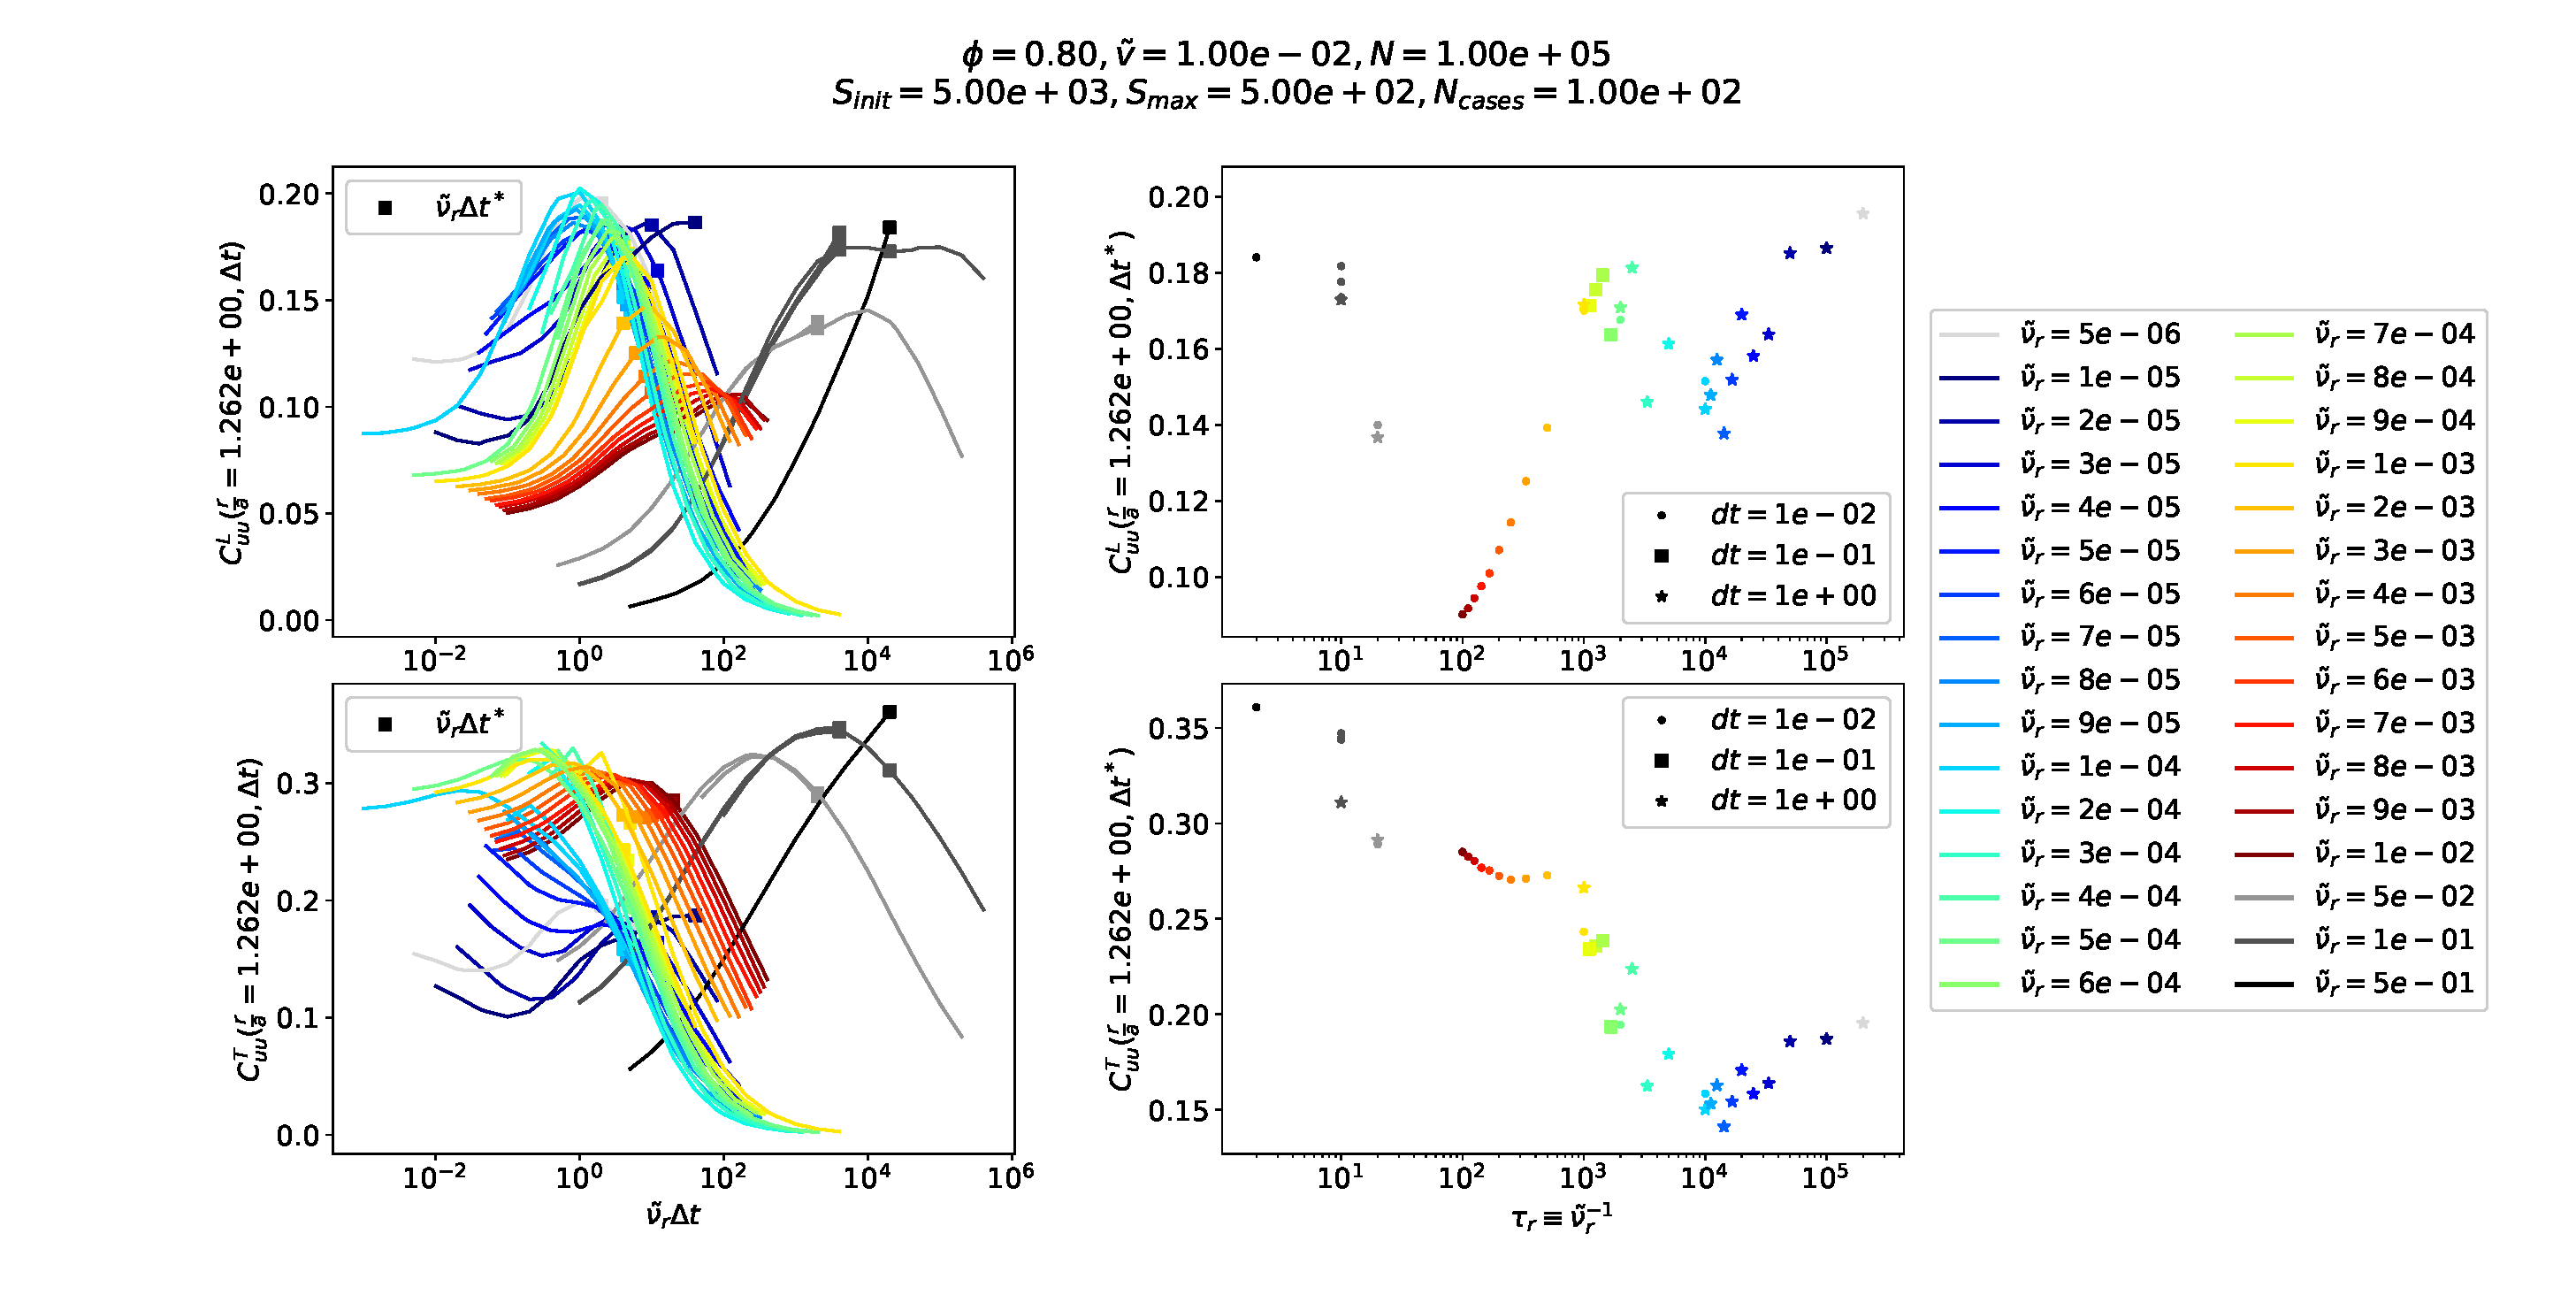
\includegraphics[width=\textwidth]{figures/figs/CuuLCuuT_Dk8000_Vj1000_Nq1000_Io5000_Mn1000_Cn5000_separate.eps}
\caption{Longitudinal and transversal displacement correlations as defined by equation \ref{cuul_cuut}, at packing fraction $\phi=0.80$ and self-propulsion velocity $\tilde{v}=1\cdot10^{-2}$, for different values of the rotational diffusion rate $\tilde{\nu}_r$. \textbf{(left)} Longitudinal (top) and transversal (bottom) displacement correlations as functions of the product of the rotational diffusion rate $\tilde{\nu}_r$ and the lag time $\Delta t$. Square markers mark the number of reorientations corresponding to the time scale of maximum cooperativity $\tilde{\nu}_r \Delta t^*$ (see figure \ref{chi_dr}). Each continuous line corresponds to a single simulation. \textbf{(right)} Longitudinal (top) and transversal (bottom) displacement correlations at times of maximum cooperativity as functions of the P\'eclet number $\text{Pe} = \tilde{v}/\tilde{\nu}_r$. Quantity $dt$ refers to the time step used in the simulation.}
\label{cuul_cuut_separate}
\end{figure}

\subsection{Varying rotational diffusion rate $\tilde{\nu}_r$}

We see in figure \ref{cuul_cuut_dr} that the ratio of transversal and longitudinal displacement correlations $C_{uu}^T/C_{uu}^L(\Delta t)$ is better behaved than the separated functions (figure \ref{cuul_cuut_separate}).\\

We observe that
\begin{itemize}
  \item at low times, this ratio has a plateau which value is greater than $1$ and increases with increasing rotational diffusion rate $\tilde{\nu}_r$ (\textit{i.e.}, decreasing persistence time $\tau_r$ and P\'eclet number $\text{Pe}$) ;
  \item at high times, this ratio is constant and equal to 1.\\
\end{itemize}

We expect the limit $\lim_{\Delta t \rightarrow +\infty} C_{uu}^T/C_{uu}^L(\Delta t) = 1$ to come from the decorrelation of the displacements of the particles at high lag times. There is no correlation in the directions of motion of pairs of particles, thus the transversal and longitudinal displacement correlations must be equal.\\

Looking at the values of the ratio at the lag time of maximum cooperativity, we note that there is a clear transition at $\text{Pe}_t \approx 10^{1.5}$ between a regime where $C_{uu}^T/C_{uu}^L(\Delta t^*) > 1$ for $\text{Pe} < \text{Pe}_t$ and a regime where $C_{uu}^T/C_{uu}^L(\Delta t^*) \approx 1$ for $\text{Pe} > \text{Pe}_t$. We note that this transition value of the P\'eclet number is consistent with the approximate transition value between the fluid states and the phase separated states inferred from the local packing fraction histogram in figure \ref{philoc_dr}, and with the transition value found in cooperativity plots in figure \ref{chi_dr_dt}.\\

We had observed in displacement maps at high activity (see figure \ref{displacement_maps}) that neighbouring particles form blocks of similar displacements, both in amplitude and direction. It follows that for these coherently moving particles, longitudinal and transversal displacement correlations are equal. This is why the value of the ratio of these correlations is equal to $1$ at lag times of maximum cooperativity in the phase separated regime.\\

In the fluid regime, figure \ref{cuul_cuut_dr} shows that displacements are mostly correlated in the transverse directions of lines joining pairs of particles.

\begin{figure}[h!]
\centering
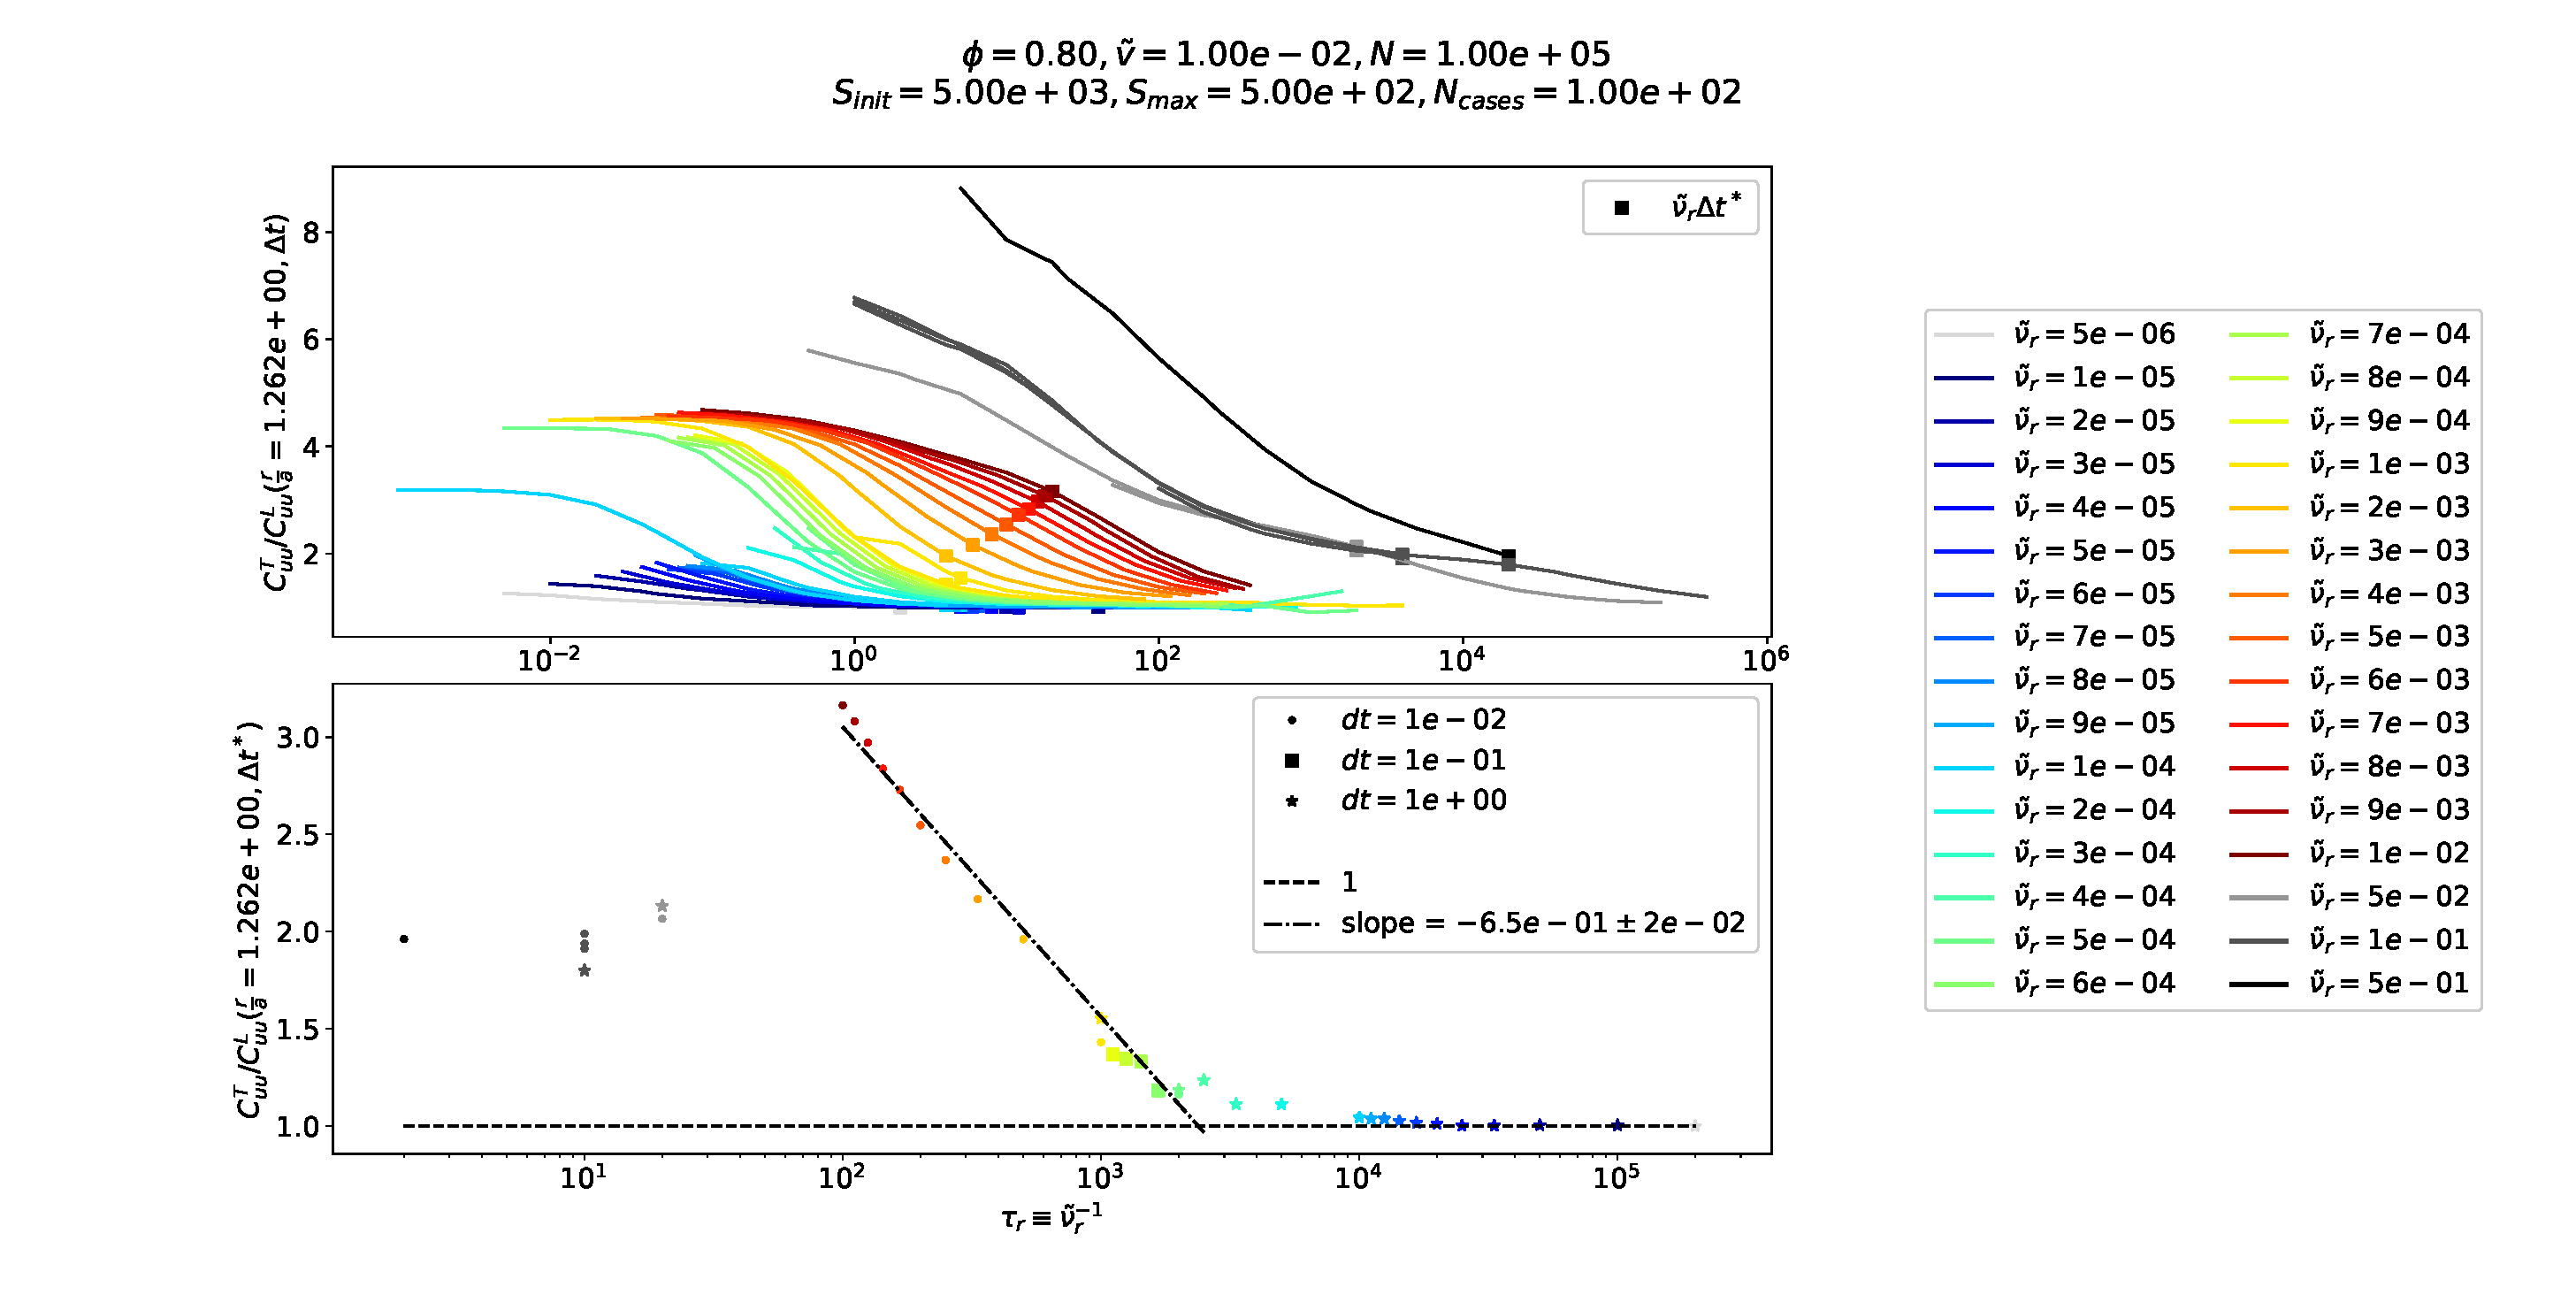
\includegraphics[width=\textwidth]{figures/figs/CuuLCuuT_Dk8000_Vj1000_Nq1000_Io5000_Mn1000_Cn5000.eps}
\caption{Ratio of transversal and longitudinal displacement correlations as defined by equation \ref{cuul_cuut}, at packing fraction $\phi=0.80$ and self-propulsion velocity $\tilde{v}=1\cdot10^{-2}$, for different values of the rotational diffusion rate $\tilde{\nu}_r$. \textbf{(top)} Ratio of transversal and longitudinal displacement correlations as function of the product of the rotational diffusion rate $\tilde{\nu}_r$ and the lag time $\Delta t$. Square markers mark the number of reorientations corresponding to the time scale of maximum cooperativity $\tilde{\nu}_r \Delta t^*$ (see figure \ref{chi_dr}). Each continuous line corresponds to a single simulation. \textbf{(bottom)} Ratio of transversal and longitudinal displacement correlations at lag time of maximum cooperativity $\Delta t^*$ as function of the P\'eclet number $\text{Pe}=\tilde{v}/\tilde{\nu}_r$. Dash-dotted line correspond to an arbitrary logarithm fit, and dashed line to $C_{uu}^T/C_{uu}^L(\Delta t^*) = 1$.}
\label{cuul_cuut_dr}
\end{figure}

\subsection{Varying self-propulsion velocity $\tilde{v}$}

We observe in figure \ref{cuul_cuut_v} that
\begin{itemize}
  \item at low times, the ratio of transversal and longitudinal displacement correlations has a plateau which value is greater than $1$ and increases with increasing self-propulsion velocity $\tilde{v}$ (\textit{i.e.}, increasing P\'eclet number $\text{Pe}$) ;
  \item at high times, this ratio is constant and equal to 1.\\
\end{itemize}

However, compared to the case of fixed $(\phi, \tilde{v})$ and varying rotational diffusion rate $\tilde{\nu}_r$ (see figure \ref{cuul_cuut_dr}), we now have that the value of the ratio at the time of maximum cooperativity $\Delta t^*$ is more or less constant and equal to $1$ for all values of the self-propulsion velocity $\tilde{v}$. There is thus no effect of the transition from the fluid regime to the phase separated regime in this particular case.

\begin{figure}[h!]
\centering
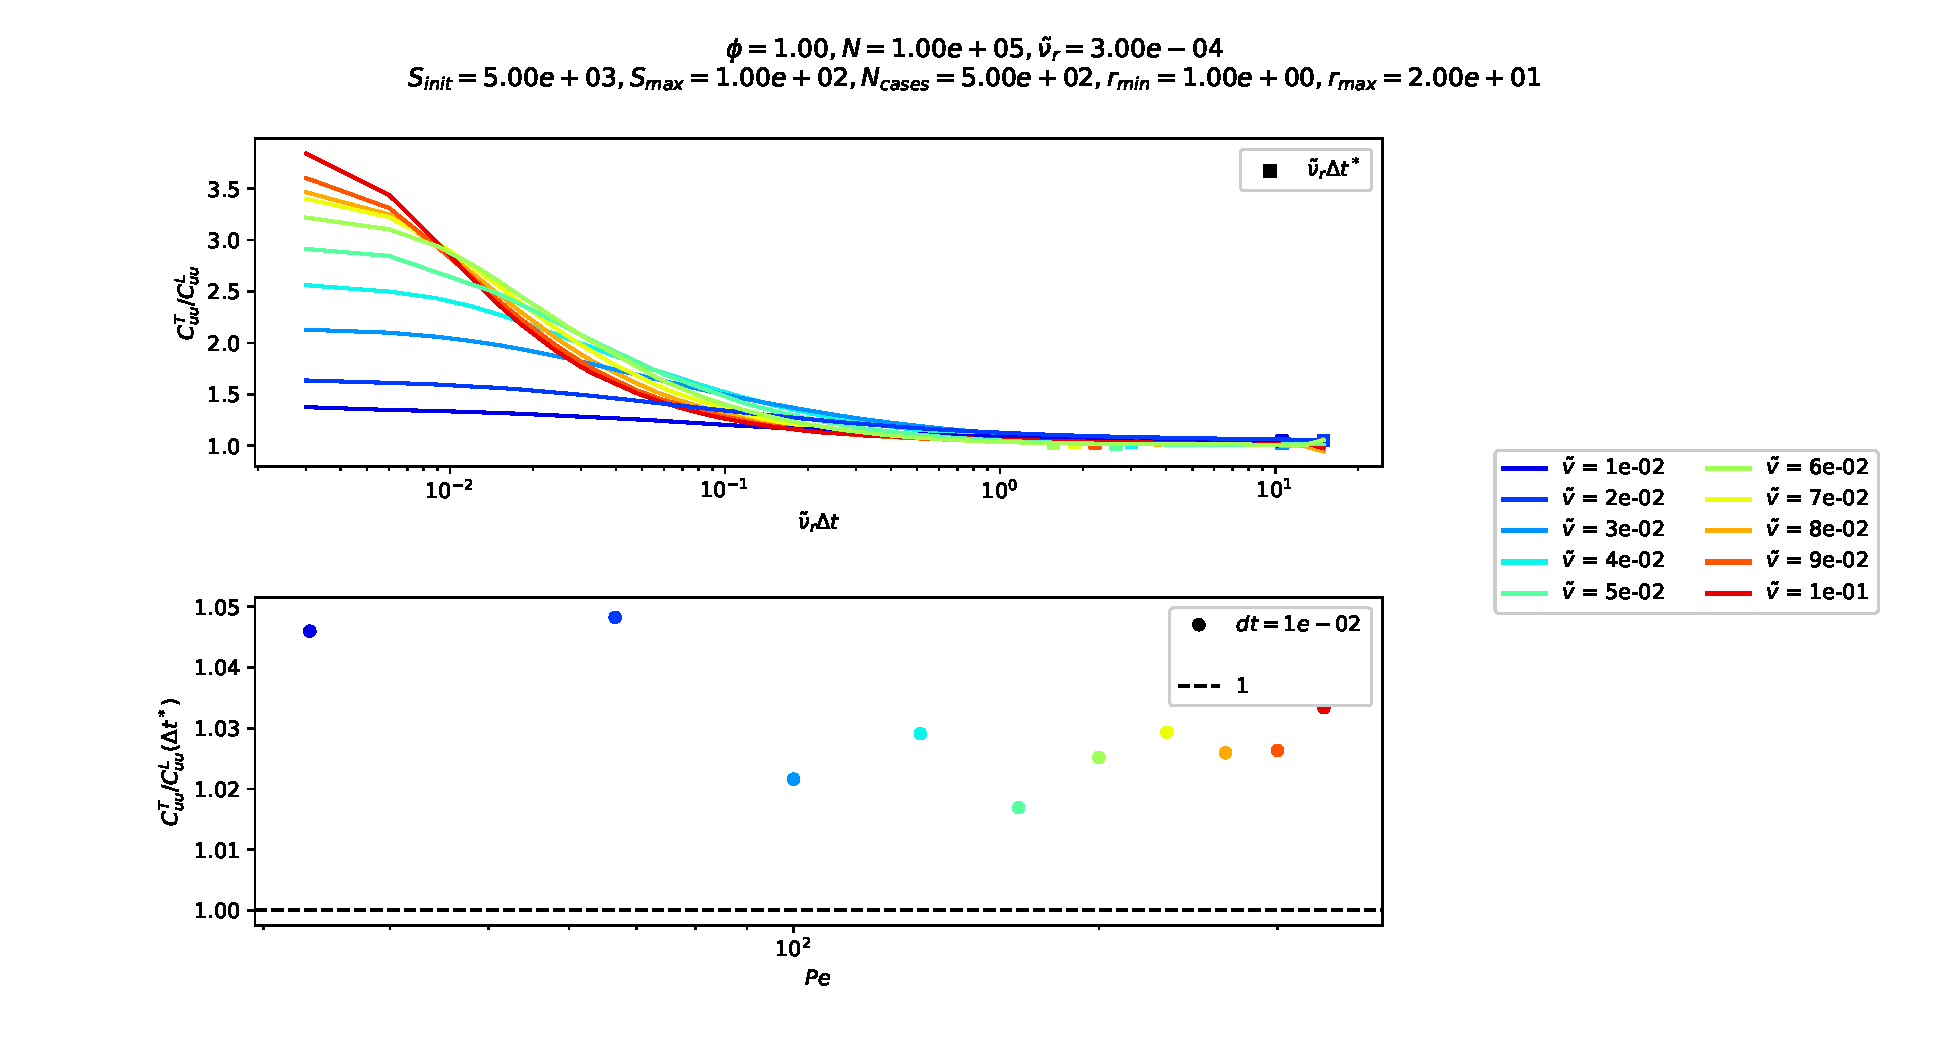
\includegraphics[width=\textwidth]{figures/figs/CuuLCuuT_Dl1000_Rh3000_Nq1000_Io5000_Mn1000_Cn5000.eps}
\caption{Ratio of transversal and longitudinal displacement correlations as defined by equation \ref{cuul_cuut}, at packing fraction $\phi=1.00$ and rotational diffusion rate $\tilde{\nu}_r=3\cdot10^{-4}$, for different values of the self-propulsion velocity $\tilde{v}$. \textbf{(top)} Ratio of transversal and longitudinal displacement correlations as function of the product of the rotational diffusion rate $\tilde{\nu}_r$ and the lag time $\Delta t$. Square markers mark the number of reorientations corresponding to the time scale of maximum cooperativity $\tilde{\nu}_r \Delta t^*$ (see figure \ref{chi_dr}). Each continuous line corresponds to a single simulation. \textbf{(bottom)} Ratio of transversal and longitudinal displacement correlations at lag time of maximum cooperativity $\Delta t^*$ as function of the P\'eclet number $\text{Pe}=\tilde{v}/\tilde{\nu}_r$. Dash-dotted line correspond to an arbitrary logarithm fit, and dashed line to $C_{uu}^T/C_{uu}^L(\Delta t^*) = 1$.}
\label{cuul_cuut_v}
\end{figure}

\newpage
\section{Overview}

We presente here comparison plots of the quantities we have introduced for the two paths in the phase diagram we have studied:
\begin{enumerate}
  \item[(i)] $(\phi = 0.80, \tilde{v} = 1\cdot10^{—2}, \tilde{\nu}_r = 1\cdot10^{—5} \rightarrow 1\cdot10^{—2})$ (figure \ref{comparison_Dk8000_Vj1000})
  \item[(ii)] $(\phi = 1.00, \tilde{v} = 1\cdot10^{—2} \rightarrow 1\cdot10^{—1}, \tilde{\nu}_r = 3\cdot10^{-4})$ (figure \ref{comparison_Dl1000_Rh3000})\\
\end{enumerate}

These plots highlight how
\begin{enumerate}
  \item[(i)] the most probable local packing fraction $\phi_{loc}^*$,
  \item[(ii)] the maximum cooperativity $\chi(\Delta t^*)$,
  \item[(iii)] the number of reorientations corresponding to the time scale of maximum cooperativity $\tilde{\nu}_r\Delta t^*$,
  \item[(iv)] and the ratio of transversal and longitudinal displacement correlations at maximum cooperativity $C_{uu}^T/C_{uu}^L(\Delta t^*)$ (only in the case of figure \ref{comparison_Dk8000_Vj1000}),
\end{enumerate}
all enable us to spot the transition between fluid and phase separated regimes.

\newpage
\subsection{Varying rotational diffusion rate $\tilde{\nu}_r$}
\vfill
\begin{figure}[h!]
\centering
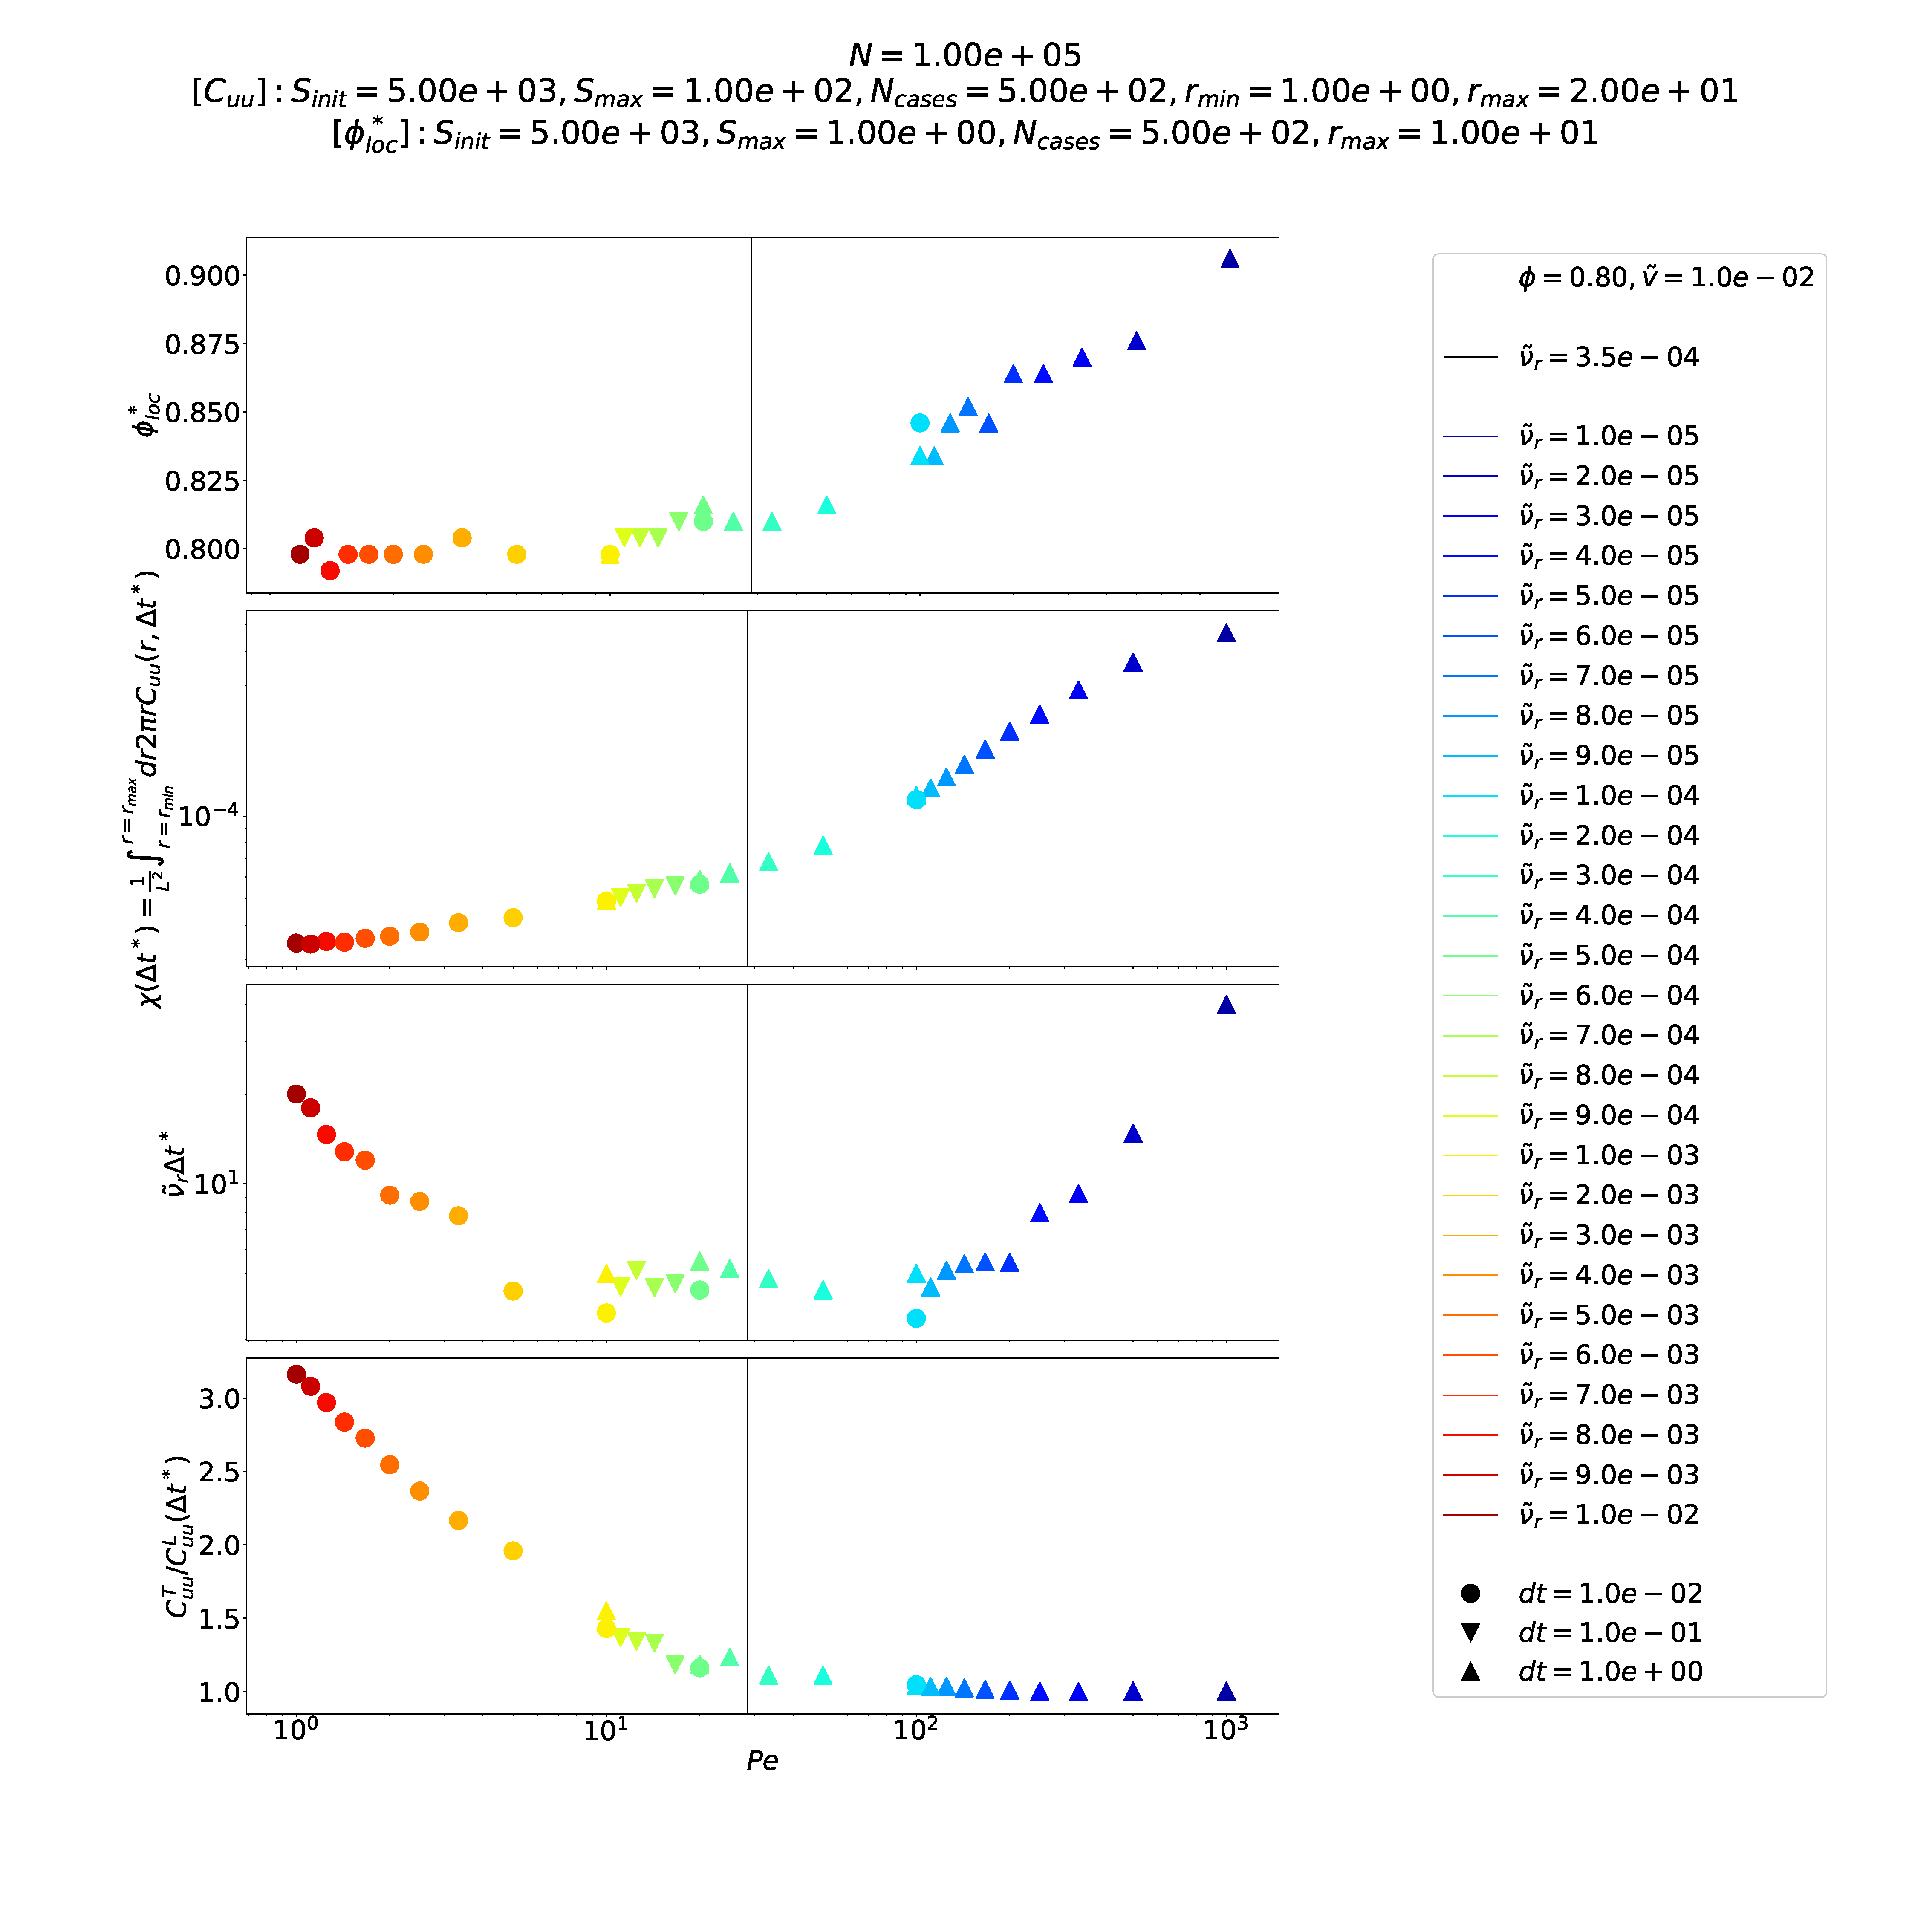
\includegraphics[width=\textwidth]{figures/figs/comparison_Dk8000_Vj1000_drdt.eps}
\caption{Comparison of \textit{(from top to bottom)} most probable local packing fraction $\phi_{loc}^*$ (see section \ref{subsection:local_density_probability}), maximum cooperativity $\chi(\Delta t^*)$ (see section \ref{section:cooperativity}), number of reorientations corresponding to the time scale of maximum cooperativity $\tilde{\nu}_r\Delta t^*$ (see section \ref{section:cooperativity}), and ratio of transversal and longitudinal displacement correlations at maximum cooperativity $C_{uu}^T/C_{uu}^L(\Delta t^*)$ (see section \ref{section:directional_displacement_correlation}), as functions of the P\'eclet number $\text{Pe} = \tilde{v}/\tilde{\nu}_r$, at packing fraction $\phi = 0.80$ and self-propulsion velocity $\tilde{v} = 1\cdot10^{—2}$. The vertical line corresponds to an arbitrarily chosen value of the transition P\'eclet number.}
\label{comparison_Dk8000_Vj1000}
\end{figure}
\vfill

\newpage
\subsection{Varying self-propulsion velocity $\tilde{v}$}
\vfill
\begin{figure}[h!]
\centering
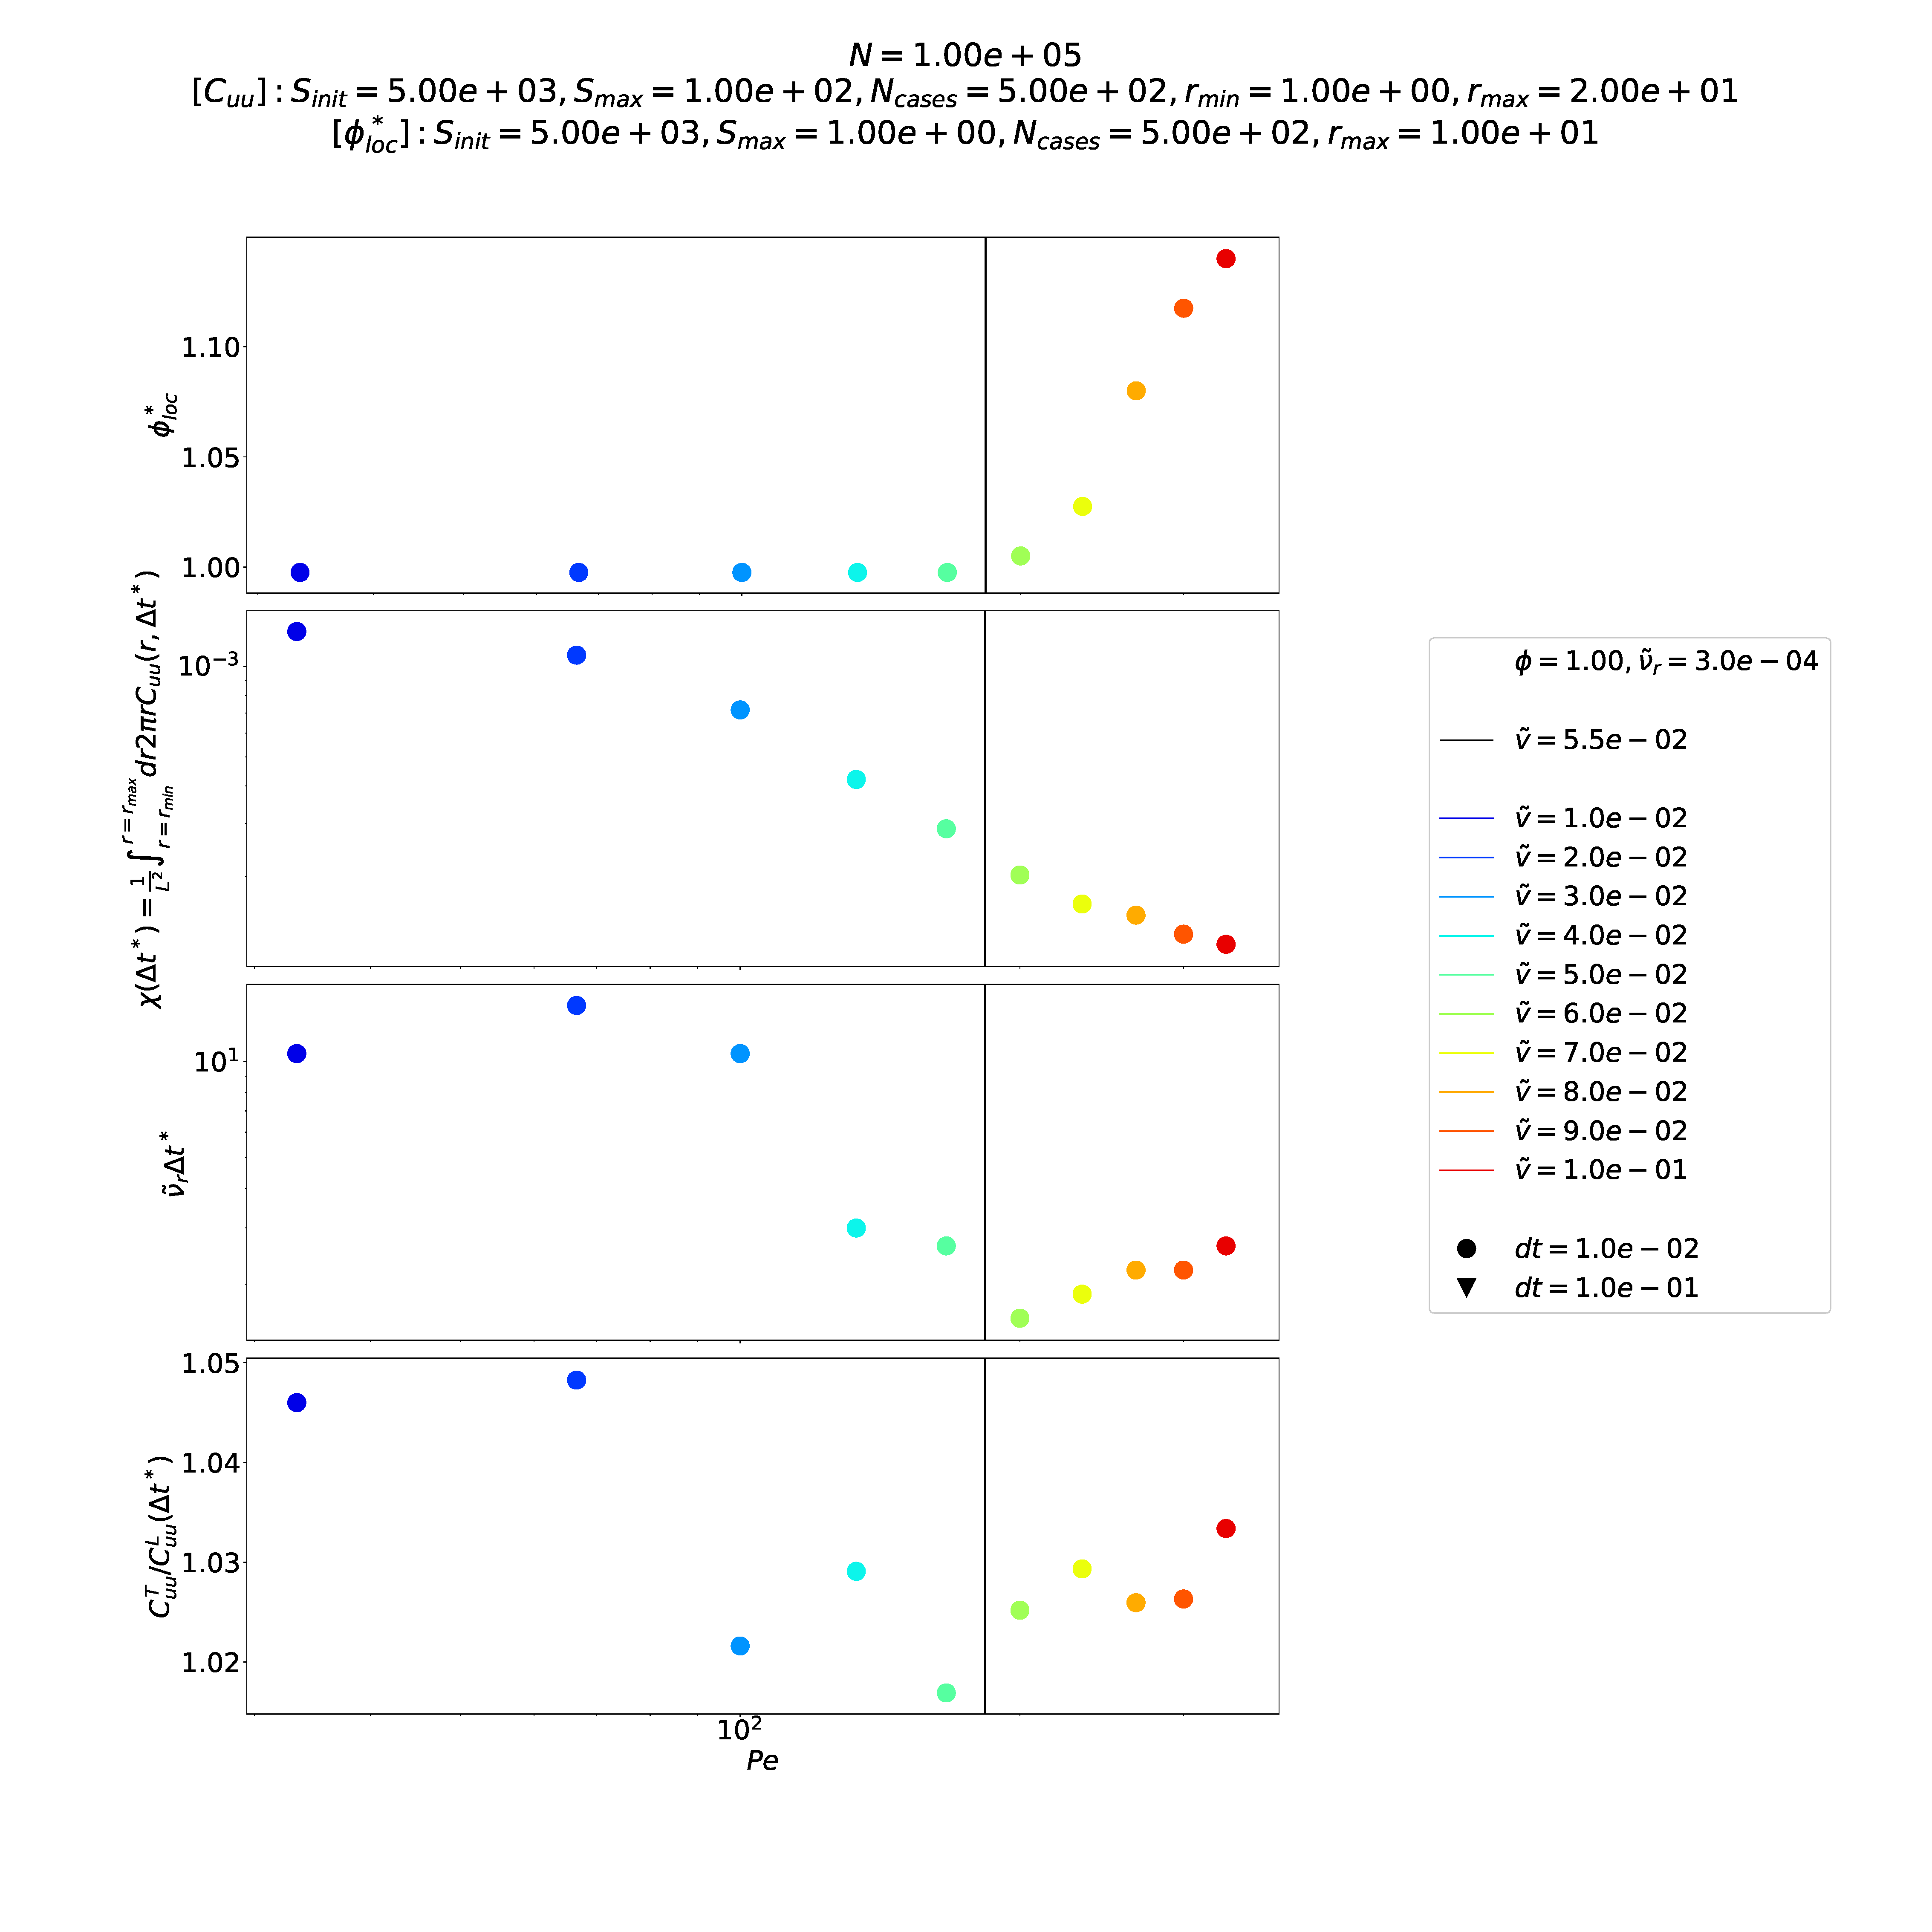
\includegraphics[width=\textwidth]{figures/figs/comparison_Dl1000_Rh3000_drdt.eps}
\caption{Comparison of \textit{(from top to bottom)} most probable local packing fraction $\phi_{loc}^*$ (see section \ref{subsection:local_density_probability}), maximum cooperativity $\chi(\Delta t^*)$ (see section \ref{section:cooperativity}), number of reorientations corresponding to the time scale of maximum cooperativity $\tilde{\nu}_r\Delta t^*$ (see section \ref{section:cooperativity}), and ratio of transversal and longitudinal displacement correlations at maximum cooperativity $C_{uu}^T/C_{uu}^L(\Delta t^*)$ (see section \ref{section:directional_displacement_correlation}), as functions of the P\'eclet number $\text{Pe} = \tilde{v}/\tilde{\nu}_r$, at packing fraction $\phi = 1.00$ and rotational diffusion rate $\tilde{\nu}_r = 3\cdot10^{—4}$. The vertical line corresponds to an arbitrarily chosen value of the transition P\'eclet number.}
\label{comparison_Dl1000_Rh3000}
\end{figure}
\vfill

\end{document}
